\documentclass[11pt,a4]{jsbook}
\setcounter{secnumdepth}{3}
\setcounter{tocdepth}{2}
\bibliographystyle{h-physrev3}
\usepackage[T1]{fontenc}
\usepackage[active]{srcltx}

\makeatletter
%\usepackage{tgtermes}
%\usepackage[T1]{fontenc}
\usepackage[top=25truemm,bottom=25truemm,left=25truemm,right=25truemm]{geometry}
\usepackage{fancyhdr, lastpage}
\usepackage{amsmath}
%\usepackage[lite,subscriptcorrection,slantedGreek,nofontinfo]{mtpro2}
\usepackage{bm,braket,ascmac,enumerate,multirow}
\usepackage{amssymb,wrapfig,afterpage,booktabs,url}
\usepackage{listings}
\usepackage[version=3]{mhchem}
\numberwithin{equation}{section}
%
\usepackage{graphicx}
\usepackage[dvips]{color}
\usepackage{makeidx}
\usepackage{fancyvrb}
\usepackage{cprotect}
\usepackage[dvipdfmx]{hyperref}
\usepackage{pxjahyper}
%
\newcommand{\vred}{\color{red}}
\newcommand{\vblue}{\color{blue}}
\newcommand{\vgreen}{\color{green}}
\newcommand{\at}{@}
%
\renewcommand{\baselinestretch}{1.1}
\renewcommand{\figurename}{Fig.}
\renewcommand{\tablename}{Table }

\makeindex 
%\renewcommand{\contentsname}{\Large \centerline{目 次}}
%\renewcommand{\figurename}{Fig.}
%\renewcommand{\tablename}{Table }
%\renewcommand{\refname}{}

\makeatother

\newcommand{ \Sec }[1]{Sec.~\ref{sec:#1}}
\newcommand{ \Appendix }[1]{Appendix \ref{sec:#1}}

\newcommand{ \Eq   }[1]{Eq.~(\ref{#1})}
\newcommand{ \Eqs  }[2]{Eqs.~(\ref{#1}) and (\ref{#2})}
\newcommand{ \Equation }[1]{Equation (\ref{#1})}

\newcommand{ \Table }[1]{Table \ref{tab:#1}}

%\newcommand{ \Ref  }[1]{Ref.~\onlinecite{#1}}
\newcommand{ \Refs }[2]{Refs.~\onlinecite{#1} and \onlinecite{#2}}

\newcommand{ \Fig     }[1]{Fig.~\ref{fig:#1}}
\newcommand{ \Figs    }[2]{Figs.~\ref{fig:#1} and \ref{fig:#2}}
\newcommand{ \Figure  }[1]{Figure \ref{fig:#1}}
%.........................................................

%.........................................................
\newtheorem{reidai}{例題}
%
\begin{document}
\title{化学工学演習I (笠原担当分)}
\maketitle
\tableofcontents
\chapter{微分方程式}
\section{常微分方程式と偏微分方程式}

\section{常微分方程式}
\subsection{初期条件,特解,一般解 –最も簡単な常微分方程式を通して–}
まずは,最も簡単な形の常微分方程式を通して,微分方程式の考え方に慣れていこう.
ここでは,下記の形の方程式を扱うことにする.
\begin{align}
 \dfrac{dy}{dx} &= g(x), \label{eq:PDE_01} 
\end{align}
$g(x)$の関数形は与えられていて,例えば$g(x) = x$などをイメージしても良い.
ここでは特定の$g(x)$の形によらない議論を行うために,$g(x)$については何も設定しない.
また,上記の方程式に加えて,$x = x_0$のときの$y$の値が分かっていて,$y\left(x_0\right) = y_{0}$であったとする.このように,微分方程式に加えて満たすべき要請を初期条件と呼ぶ.
微分方程式を解くということは,その与えられた方程式と条件を満たす関数$y\left(x\right)$を
求める,ということを意味する.

最初なので,丁寧に式変形を示していくことにする.
まず,式中の$x$を$x^\prime$と置き換えておく.
%
\begin{align}
 \dfrac{dy}{dx^{\prime}} & =g\left(x^{\prime}\right).
\end{align}
%
両辺を,
$x^{\prime}$について$x_0$から$x$まで積分する.
\begin{align}
 \int_{x_{0}}^{x}dx^{\prime}\,\dfrac{dy}{dx^{\prime}} & =\int_{x_{0}}^{x}dx^{\prime}\,g\left(x^{\prime}\right). \label{eq:PDE_01_teiseki}
\end{align}
そうすると,左辺は
\begin{align}
 \int_{y\left(x_{0}\right)}^{y\left(x\right)}dy & =y\left(x\right)-y_{0},
\end{align}
と書き直せる.右辺については,$g(x^\prime)$の形が具体的に与えられないことには
積分を実行できないので,そのままにしておく.つまり,
\begin{align}
 y = \int_{x_0}^{x} dx^\prime \, g(x^\prime) + y\left(x_0\right), \label{eq:PDE_01_sol_01}
\end{align}
という形で$y$の表式が得られる.これが\Eq{eq:PDE_01}の解である.

本テキストでは,定積分\Eq{eq:PDE_01_teiseki}を実行することで,
微分方程式の解を求めた.教科書の多くでは,
不定積分を用いた形で解の形を出しているかもしれない.
その場合は,積分定数$C$を用いて,
\begin{align}
y & =\int dx\, g\left(x\right)+C, \label{eq:PDE_01_sol_02}
\end{align}
と表される.$C$は初期条件によって決まる定数(任意定数)である\footnote{本テキストでは,断りなく$C$と書いたときは,積分定数を表すことにする.}.
つまり,この微分方程式において初期条件の違いは全て定数$C$の値に反映される.実際,\Eq{eq:PDE_01_sol_01}と\Eq{eq:PDE_01_sol_02}を見比べると,
$C=y_0$であることが分かる.
\Eq{eq:PDE_01_sol_02}は,考えうる全ての初期条件に対応できる解の形になっており,そのような解のことを一般解と呼ぶ.
そして,無数にある解の一つのことを,一般解と区別して特解と呼ぶ.
このテキストでも,以後は不定積分を用いた形で一般解を表していくことにする.

言うまでもないことかもしれないが,
自身が導き出した解が,本当に微分方程式の解になっているかどうか
は簡単に確認できるということはちゃんと認識しておくべきであろう.
今回の場合では,\Eq{eq:PDE_01_sol_02}を\Eq{eq:PDE_01}に代入すると,
\begin{align}
  \dfrac{d}{dx}\left(\int dx\,g\left(x\right)+C\right) & =g\left(x\right),
\end{align}
となり,確かに微分方程式の解になっていることが分かる.
このように,解を導出した後に確認する習慣を身につけておけば,
思わぬケアレスミスを防ぐことが出来る.
%
\subsection{物理・化学でよく現れる常微分方程式}
%
微分方程式の教科書では,
初めのうちに常微分方程式をその形に応じて分類していることが多い(例えば線形 or 非線形など).
本テキストでは,
まずは初等的な物理・化学でよく現れる常微分方程式の解法について
一つ一つ学び,その後にそれらの方程式がどのように分類されるかを学んでいくことにする.

\subsubsection{$\dfrac{dy}{dx} + a y = 0$}
%
次の形の微分方程式を考える.
\begin{align}
 \dfrac{dy}{dx} + a y = 0. \label{eq:PDE_02} 
\end{align}
$y\neq 0$のとき,両辺を$y$で割る.
\begin{align}
\dfrac{1}{y}\dfrac{dy}{dx} = -a. 
\end{align}
両辺を積分すると左辺は
\begin{align}
 \int dx\,\dfrac{1}{y}\dfrac{dy}{dx} 
 & = \int dx\,\dfrac{d}{dx}\log \left|y\right|, 
\end{align}
だから,
\begin{align}
\log \left| y \right| = -ax + C,\\
\left| y \right| = e^{C} e^{-ax}, 
\end{align}
である.$A>0$として,
$y> 0 $のときは$e^C \to A$, $y < 0$のときは$e^{C} \to -A$と置き換えれば良い.
また,$y=0$も明らかに解であるが,これは$A=0$に対応している.
従って,いずれの場合においても,
\begin{align}
 y = C e^{-ax}, 
\end{align}
と表すことが出来る.ただし,これまでの慣習に従って
任意定数を$A$ではなく$C$で表している.
 
%
\subsubsection{$\dfrac{dy}{dx} + a y = g(x)$\label{sec:PDE_03}}
%
次の形の常微分方程式を考える.
\begin{align}
 \dfrac{dy}{dx} + a y = g(x). \label{eq:PDE_03}
\end{align}
%\Eq{eq:PDE_01}とは異なり,単純に両辺を積分しても上手くいかない.
%実際にやってみると,
%\begin{align}
%  y+a\int dx^{\prime}\,y & =\int dx^{\prime}\,g\left(x^{\prime}\right)+C, \label{eq:PDE_02}
%\end{align}
%となり,左辺に未知関数$y$の積分が残ってしまい,これ以上式変形を進められなくなってしまう.
%今,私たちが解の求め方を知っているのは\Eq{eq:PDE_01}の形をした方程式のみである.そこで,
\Eq{eq:PDE_02}を式変形して\Eq{eq:PDE_01}の形に書き換えることを考えてみる.
まず,\Eq{eq:PDE_01}の両辺に何らかの関数$f\left(x\right)$をかけてみる.
\begin{align}
 f\left(x\right)\dfrac{dy}{dx}+af\left(x\right)y&=f\left(x\right)g\left(x\right). \label{eq:PDE_03_01}
\end{align}
もし左辺が
\begin{align}
 f\left(x\right)\dfrac{dy}{dx}+af\left(x\right) & =\dfrac{d}{dx}\left(f\left(x\right)y\right), \label{eq:PDE_03_lhs}
\end{align}
の形でまとめられると都合が良い.
というのも,$Y=f\left(x\right)y$とおくと,\Eq{eq:PDE_03}は
\begin{align}
 \dfrac{dY}{dx} & =f\left(x\right)g\left(x\right), 
\end{align}
となり,既に解法を知っている\Eq{eq:PDE_01}の形に帰着するからだ.
従って,\Eq{eq:PDE_03_lhs}を満たす$f\left(x\right)$を見つければ良い.積の微分法より,
\begin{align}
 \dfrac{d}{dx}\left(f\left(x\right)y\right)=f\left(x\right)\dfrac{dy}{dx}+\left(\dfrac{d}{dx}f\left(x\right)\right)y, 
\end{align}
であるから,\Eq{eq:PDE_03_lhs}の左辺と比較すると,$f\left(x\right)$は
\begin{align}
 \dfrac{df\left(x\right)}{dx} = af\left(x\right),
\end{align}
を満たせば良い.この$f\left(x\right)$に対する微分方程式の解(の一つ)は
\begin{align}
  f\left(x\right) = e^{ax},
\end{align}
である.従って,\Eq{eq:PDE_03}は,
\begin{align}
  \dfrac{d}{dx}\left(e^{ax}y\right) & =e^{ax}g\left(x\right).
\end{align}
と書き直すことが出来るので,一般解は
\begin{align}
  e^{ax}y & =\int dx\,e^{ax}g\left(x\right)+C, \\
  y & =e^{-ax}\int dx\,e^{ax}g\left(x\right)+Ce^{-ax},
\end{align}
である.
%
\subsubsection{$\dfrac{d^2y}{dx^2} + a \dfrac{dy}{dx} + by = 0$\label{sec:PDE_04}}
%
微分方程式
\begin{align}
  \dfrac{d^2y}{dx^2} + a \dfrac{dy}{dx} + by = 0, \label{eq:PDE_04}
\end{align}
は,2階微分を含んでおり,これまで見てきた微分方程式よりも複雑そうに見えるが,
実は少し式変形することで,\Eq{eq:PDE_03}の形に直すことが出来る.まず,
\begin{align}
  \dfrac{d^{2}y}{dx^{2}}+a\dfrac{dy}{dx}+by & =\dfrac{d}{dx}\left(\dfrac{dy}{dx}-py\right)-q\left(\dfrac{dy}{dx}-py\right),
\end{align}
と表すことを考える.$Y = dy/dx - py$とおけば,これは元々の式を
\begin{align}
  \dfrac{dY}{dx} - qY = 0, \label{eq:PDE_04_convert} 
\end{align}
の形に書き換えたことになる.
\begin{align}
  \dfrac{d}{dx}\left(\dfrac{dy}{dx}-py\right)-q\left(\dfrac{dy}{dx}-py\right) & =\dfrac{d^{2}y}{dx^{2}}-\left(p+q\right)\dfrac{dy}{dx}+pqy.
\end{align}
元々の方程式と係数を比較すると,$p,~q$は
\begin{align}
  \begin{cases}
    p + q &= -a \\
    pq    &= b 
  \end{cases},
\end{align}
である.つまり,$p,~q$は
\begin{align}
  \left(\lambda-p\right)\left(\lambda-q\right) & =\lambda^{2}-\left(p+q\right)\lambda+pq\notag\\
   & =\lambda^{2}+a\lambda+b\notag\\
   & =0,
\end{align}
で表される$\lambda$に関する2次方程式の解である.
このようにして得られる2次方程式を特性方程式と呼ぶ.
\Eq{eq:PDE_04_convert}を解くと,
\begin{align}
  \dfrac{dy}{dx} - py & = C_{1}e^{qx},
\end{align}
であり,この形の微分方程式は\Eq{eq:PDE_03}と同じなので,
\begin{align}
y = C_{1}e^{px}\int dx\, e^{\left(q-p\right)x} + C_{2}e^{px}, \label{eq:PDE_04_sol_general} 
\end{align}
である.
ここからは$p = q$と$p\neq q$ の場合に分けて式変形を進める.
まず,$p=q$の場合,\Eq{eq:PDE_04_sol_general}より,
\begin{align}
  y &= C_{1}e^{px}\int dx + C_{2}e^{px} \notag \\
    &= C_{1} x e^{px} + C_{2}e^{px},
\end{align}
である.次に,$p \neq q$ の場合では,\Eq{eq:PDE_04_sol_general}内の積分を実行して,
\begin{align}
 y = \dfrac{C_{1}}{q-p} e^{qx} + C_{2}e^{px},
\end{align}
と書ける.$C_1/\left(q -p \right)$を改めて$C_{1}$とおいて,
\begin{align}
 y = C_{1} e^{qx} + C_{2}e^{px}, 
\end{align}
と書き直しても良い.
$p,~q$が虚数の場合,実数$\alpha,~\beta$を用いて,
\begin{align}
  p &= \alpha + i \beta, \\
  q &= \alpha - i \beta, 
\end{align}
と表すことにすれば,
\begin{align}
  y = C_{1}e^{\alpha x}e^{i\beta x} + C_{2}e^{\alpha x}e^{-i\beta x},
\end{align}
である.オイラーの公式を用いれば三角関数を用いた表現に直せるが,その導出は各自に委ねることとする.

これまでに出てきた微分方程式とは異なり,
今回の微分方程式\Eq{eq:PDE_04}の一般解には
2つの任意定数が現れている.これは,これまでの微分方程式が1階の微係数だけを
含んでいたのに対し,\Eq{eq:PDE_04}では2階の微係数が含まれているためである\footnote{後に用語としてまとめるが,$n$階の微係数を含む常微分方程式のことを$n$階常微分方程式と呼ぶ.}.
このように微分方程式に含まれる階数と任意定数の数は対応している.

最後に,特性方程式について触れておく.
この2次方程式は\Eq{eq:PDE_04}の微係数を
\begin{align}
 \dfrac{d^{2}y}{dx^{2}} & \to \lambda^{2}, \\
 \dfrac{dy}{dx}         & \to \lambda, 
\end{align}
に置き換えた形になっている.
少し別のアプローチから特性方程式を導き出そう.
微分方程式\Eq{eq:PDE_04}の形を見て,
$e^{\lambda x}$が解になりそうだと予想し代入してみる.すると,
\begin{align}
  \dfrac{d^{2}}{dx^{2}}\left(e^{\lambda x}\right)+a\dfrac{d}{dx}\left(e^{\lambda x}\right)+be^{\lambda x} & =\left(\lambda^{2}+a\lambda+b\right)e^{\lambda x}\notag \\
 & =0,
\end{align}
つまり
\begin{align}
  \lambda^2 + a \lambda + b = 0, 
\end{align}
が得られるが,これは特性方程式である.
従って,特性方程式の解となる$\lambda$の値を用いれば,
$e^{\lambda x}$は微分方程式の解となる.
特性方程式が2つの解$\lambda_1,~\lambda_2$を持つ場合は,
特解$e^{\lambda_1 x}$,$e^{\lambda_2 x}$の線形結合で
一般解を構成できる\footnote{特性方程式が重解を持つ場合は,特性方程式からは
特解が1つしか得られないので,一般解を出すためにはもう一つ特解を求める必要があるが,後で学ぶ定数変化法を用いると,簡単に求めることができる.}.

%
\subsubsection{$\dfrac{dy^2}{dx^2} \pm \beta^2 y =0$}
$\beta$は実数として,
\begin{align}
  \dfrac{d^2 y}{dx^2} - \beta^{2}y = 0, \label{eq:PDE_05_01}
\end{align}
を考える.
特性方程式は,
\begin{align}
  \lambda^2 -\beta^2 = 0,
\end{align}
なので,$\lambda = \pm \beta$である.従って,
\begin{align}
  y = C_{1} e^{-\beta x} + C_{2} e^{\beta x},
\end{align}
である.

次に,
\begin{align}
  \dfrac{d^2 y}{dx^2} + \beta^{2} y = 0, \label{eq:PDE_05_02}
\end{align}
を考える.特性方程式
\begin{align}
  \lambda^2 + \beta^2 = 0,
\end{align}
より,$\lambda = \pm i\beta$だから,
\begin{align}
  y = C_1 e^{-i\beta x} + C_{2} e^{i\beta x}, \label{eq:PDE_05_02_sol_01} 
\end{align}
である.オイラーの公式
\begin{align}
  e^{\pm i a} = \cos a \pm i\sin a, 
\end{align}
を用いると,
\begin{align}
  y & =  C_{1}\left(\cos \beta x - i \sin \beta x\right) 
       + C_{2}\left(\cos \beta x + i \sin \beta x\right) \notag \\
    & =  \left(C_1 + C_2 \right)\cos \beta x + i (C_2 - C_1) \sin \beta x,
\end{align}
である.従って,三角関数の係数を改めて$C_1,~C_2$と置き直して,
\begin{align}
  y = C_1 \cos \beta x + C_2 \sin \beta x, \label{eq:PDE_05_02_sol_02}
\end{align}
と表すことが出来る.
導出過程を見れば分かるとおり,\Eq{eq:PDE_05_02_sol_01}と\Eq{eq:PDE_05_02_sol_02}のどちらも正しい一般解である.
%
\subsection{常微分方程式の分類}
\subsubsection{線形と非線形}
$x$を引数とする関数$y\left(x\right)$に関する常微分方程式を考える.
微係数$\left\{d^{i}y/dx^{i}\right\}$の1次式で表された常微分方程式を
線形微分方程式と呼ぶ.式の中に含まれる最大階数が$n$のとき,その常微分方程式を
$n$階常微分方程式と呼び,一般に次式のように表される.
\begin{align}
a_{n}\left(x\right)\dfrac{d^{n}y}{dx^{n}}+a_{n-1}\left(x\right)\dfrac{d^{n-1}y}{dy^{n-1}}+\cdots+a_{1}\left(x\right)\dfrac{dy}{dx}+a_{0}\left(x\right) y & =b\left(x\right).
\end{align}
このテキストでこれまで扱ってきた常微分方程式は全て線形である.
この形で表せない常微分方程式のことを非線形常微分方程式と呼ぶ.
例えば,
\begin{align}
  \dfrac{d^{2}y}{dx^{2}} & =-a\sin y, \label{eq:PDE_general}
\end{align}
は$y\left(x\right)$が三角関数の引数になっているため非線形微分方程式である.
このような非線形微分方程式を解析的に解くことは極めて難しく,
実際に解ける例は僅からしい.
そのため,非線形微分方程式の解の振る舞いを調べる研究は,
数学や数理物理における最先端の一つであるようだ.
従って,このテキストで取り扱うのは主に線形とする.

%
\subsubsection{斉次と非斉次}
%
線形常微分方程式\Eq{eq:PDE_general}において,
$b(x) = (定数)$のとき,斉次線形常微分方程式と呼び,
$b(x) \neq (定数)$のとき,非斉次線形常微分方程式と呼ぶ.
従って,これまで扱った方程式を斉次か非斉次かで分類すると以下のようになる.
\begin{align}
  &\text{\Eq{eq:PDE_01}}\quad  \dfrac{dy}{dx} = g(x) \text{ : 斉次}\\
  &\text{\Eq{eq:PDE_02}}\quad  \dfrac{dy}{dx} + a y = 0 \text{ : 斉次} \\
  &\text{\Eq{eq:PDE_03}}\quad  \dfrac{dy}{dx} + ay = g(x) \text{ : 非斉次} \\
  &\text{\Eq{eq:PDE_04}}\quad  \dfrac{d^2y}{dx^2} + a \dfrac{dy}{dx} + by = 0 \text{ : 斉次}
\end{align}
容易に想像がつくが,非斉次方程式の解を求める方が斉次の場合よりも一般解を求めるのが難しくなるが,
代表的な形の微分方程式については,解法が確立されている.
%
\subsection{線形常微分方程式に関する基本的な定理}
%
\subsubsection{斉次形 : 解の線形結合もまた解}
%
\begin{shadebox}
斉次形の$n$階線形常微分方程式
\begin{align}
 \sum_{i=0}^{n}a_{i}\left(x\right)\dfrac{d^{i}y}{dx^{i}}& =0, 
\label{eq:homo_linear}
\end{align}
の解を$y_1,~y_2$とすると,その線形結合
\begin{align}
  y\left(x\right) = C_{1}y_{1} + C_{2}y_{2},  \label{eq:homo_linear_comb_sol}
\end{align}
もまた解である.
\end{shadebox}
%
ここまでで経験してきた微分方程式の解の導出を考えれば,
定理として証明するまでもないかもしれないが,一応証明しておく.
\Eq{eq:homo_linear}の左辺に\Eq{eq:homo_linear_comb_sol}を代入すると,
\begin{align}
 \sum_{i=0}^{n}a_{i}\left(x\right)\dfrac{d^{i}}{dx^{i}}\left(C_{1}y_{1}+C_{2}y_{2}\right) & =C_{1}\left(\sum_{i=0}^{n}a_{i}\left(x\right)\dfrac{d^{i}y_{1}}{dx^{i}}\right)+C_{2}\left(\sum_{i=0}^{n}a_{i}\left(x\right)\dfrac{d^{i}y_{2}}{dx^{i}}\right),
\end{align}
$y_1,~y_2$は微分方程式の階であるから,右辺の括弧内はゼロになるので,
確かに\Eq{eq:homo_linear_comb_sol}は微分方程式の解になっていることが分かる.
%
\subsubsection{斉次形 : $n$階微分方程式の一般解の形}
%
斉次の$n$階線形常微分方程式の一般解について,
証明なしに述べる.これは,
\Sec{PDE_04}で述べた事項の一般化に当たる.
%
\begin{shadebox}
 斉次の$n$階線形常微分方程式
\begin{align}
 \sum_{i=0}^{n}a_{i}\left(x\right)\dfrac{d^{i}y}{dx^{i}}& =0, 
\end{align}
の一般解は,$n$個の線形独立な特殊解$\left\{y_i\right\}$の線形結合
\begin{align}
  y & =\sum_{i=1}^{n}C_{1}y_{1},
\end{align} 
で表される.
\end{shadebox}

\subsubsection{非斉次形 : 非斉次形の一般解は,斉次形の一般解と非斉次形の特殊解の和}
\begin{shadebox}
非斉次の$n$階線形常微分方程式
\begin{align}
 \sum_{i=0}^{n}a_{i}\left(x\right)\dfrac{d^{i}y}{dx^{i}} & =b\left(x\right), \quad b\left(x\right) \neq \mathrm{Const.}
\label{eq:inhomo_linear}
\end{align}
の特殊解を$y_s$, 対応する斉次形
\begin{align}
 \sum_{i=0}^{n}a_{i}\left(x\right)\dfrac{d^{i}y}{dx^{i}} & = 0,
\end{align}
の一般解を$y_h$とすると,\Eq{eq:inhomo_linear}の一般解は
\begin{align}
  y = y_{h} + y_{s}, \label{eq:inhomo_linear_sol}
\end{align}
で表される.
\end{shadebox}
%
\Eq{eq:inhomo_linear}に,\Eq{eq:inhomo_linear_sol}を代入すると,
\begin{align}
 \sum_{i=0}^{n}\dfrac{d^{i}}{dx^{i}}\left(y_{h}+y_{s}\right) & =\sum_{i=0}^{n}a_{i}\left(x\right)\dfrac{d^{i}y_{h}}{dx^{i}}+\sum_{i=0}^{n}a_{i}\left(x\right)\dfrac{d^{i}y_{s}}{dx^{i}}\notag\\
 & =0+b\left(x\right)\notag\\
 & =b\left(x\right), 
\end{align}
となるので,確かに\Eq{eq:inhomo_linear_sol}は非斉次形の解になっている.これが一般解であるかどうかを確認する必要があるが,
これは本テキストの範疇を超えるので,省略することにする.

この定理は非斉次の線形常微分方程式を解く上で有用な定理である.
というのも,比較的簡単に解ける斉次方程式の一般解と,
どんな方法でも良いので非斉次方程式の特殊解を一つでも見つけさえすれば,
その2つから非斉次方程式の一般解を求められたことになるからだ.
そこで,この後は斉次方程式の一般解を求める方法をいくつか学んだ後,
非斉次方程式の特殊解を探し出す方法について述べる.

%
\subsection{変数分離}
%
1階微分方程式のうち,
\begin{align}
  \dfrac{dy}{dx} & =f\left(y\right)g\left(x\right),
\end{align}
の形をしたものを,変数分離形と呼ぶ.$f\left(x\right) \neq 0$のとき,
両辺を$f\left(x\right)$で割り,
\begin{align}
  \dfrac{1}{f\left(y\right)}\dfrac{dy}{dx} = g\left(x\right),
\end{align}
とした後,$x$について積分することで解を得ることが出来る.
変数分離形の最もシンプルな例は,\Eq{eq:PDE_02}である.
\begin{align}
 \dfrac{dy}{dx} + ay = 0. 
\end{align}
確認してみると分かるが,
この方程式の解を解くときにも,上記の手続きを踏んでいる.

\subsubsection{同次形}
%
1階の微分方程式が
\begin{align}
  \dfrac{dy}{dx} = f\left(\dfrac{y}{x}\right),
\end{align}
の形であるとき,この微分方程式のことを同次形と呼ぶ.
同次形の場合,変数変換により変数分離形に書き直すことが出来る.
まず,$y=u\left(x\right)x$とおくと,
\begin{align}
 x\dfrac{du\left(x\right)}{dx}+u\left(x\right) & =f\left(u\left(x\right)\right),
\end{align}
だから,$f\left(u\right) - u\left(x\right) \neq 0$のとき,
\begin{align}
 \dfrac{1}{f\left(u\left(x\right)\right)-u\left(x\right)}\dfrac{du\left(x\right)}{dx}=\dfrac{1}{x},
\end{align}
と出来るので,確かに変数分離形になっている.
%
\subsection{定数変化法}

\subsection{未定係数法}
\setcounter{chapter}{1}
\chapter{フーリエ解析入門}
%
波動や振動現象など,何らかの系の状態を表す関数が周期的に振る舞うものは
私たちの身の周りに溢れている.
例えば,私たちに近い分野でみると,
種々の分光学的測定で得られる時系列データ(信号)は周期関数(とみなせるもの)である.
それらは一見するとグチャグチャしていて,ただ漠然と眺めているだけでは新しい知見は得られない.
そうではなく,例えば,その信号の中にはどういった振動数の波がどの程度含まれているか,
などを取り出すことが出来れば,その現象の理解を深めることができる.
その要求に答える数学的手法がフーリエ (Fourier)解析である.
この例に限らず,フーリエ解析は極めて広い分野で使われる強力な手法であり,
前章で学んだ微分方程式を解く際にも有効である.
そこで,この章ではフーリエ解析について学んでいくことにする.
ただし,「フーリエ解析」という名前で1期分の講義があるくらいで,
フーリエ解析に関する諸事項を幅広くかつ厳格に述べるには圧倒的に時間が足りないので,
かなり初歩的な事項を紹介するに留めざるを得ないが,それでも応用範囲は広い.

%しかし,
%ここでは,近い将来皆さんが化学工学の分野で研究を進めていてフーリエ解析
%の知識が必要に
%
\section{フーリエ級数}
%
皆さんにとって馴染みのあるテイラー展開について考えてみよう.
テイラー展開とは,次式のように
関数$f(x)$をべき級数として展開する,というものであった.
\begin{align}
  f\left(x\right) &= f\left(a\right) + f^{\prime}\left(a\right)
 \left(x-a\right) + \dfrac{f^{\prime\prime}\left(a\right)}{2!}\left(x-a\right)^{2} + \cdots. 
\end{align}
%
上述のように,テイラー展開ではべき級数となるが,$x^{0},~x^{1},~x^2,~x^3,\cdots$以外にも,何らかの関数のセットで展開出来るのではないか
と考えることは,一般性を重んじる(ことが多い)数学の立場からすると自然なことである.実際,そのような関数のセットを系統立てた考えの元に
用意することは可能で\footnote{このあたりの話はとても面白いのだが,時間の都合上省略する.興味が出た人は直交関数やグラム-シュミットの直交化法といったキーワードで調べてみると良い.決して難しくはない.},
関数のセットの一つとして,三角関数(sin, cos)が挙げられる.
周期関数を展開する際に,三角関数を用いるのはもっともらしいように思える.実は周期関数を三角関数を用いて展開して得られるものをフーリエ級数と呼び,これから学んでいくことになる.

まずは,周期関数について整理しておく.
周期$L~(>0)$の関数$f(x)$とは,
\begin{align}
  f\left(x + L\right) = f\left(x\right), 
\end{align}
を満たす関数のことを指す.
また,もし$a\leq x \leq b$の範囲で定義されている関数の場合は,
それを周期$b-a$の周期関数と一部とみなして,全区間に拡張することができる.
%
\begin{figure}[htbp]
  %\includegraphics[width=1.0\linewidth]{figures/extend_function.eps} 
  \includegraphics[width=1.0\linewidth]{/Users/kasa/GitHub/lectures/osaka-u/2021/kaenI/chap02_fr/figures/extend_function.eps} 
\end{figure}
%
\subsection{三角関数に関する諸公式}
%
フーリエ解析で現れる式変形では,割と高い頻度で高校数学で学んだタイプの三角関数の定理や積分
が現れる.それをその都度証明していくのは大変なので,ここで公式としてまとめておく.
\begin{align}
 &\sin\left(\alpha \pm \beta\right) = \sin\alpha \cos \beta \pm \cos\alpha \sin\beta, \\
 &\cos\left(\alpha \pm \beta\right) = \cos\alpha \cos \beta \mp \sin\alpha \sin\beta, \\
 &\sin^{2} \alpha = \dfrac{1-\cos 2\alpha}{2}, \\
 &\cos^{2} \alpha = \dfrac{1+\cos 2\alpha}{2}, \\
 &\sin \alpha \cos \beta = \dfrac{1}{2}\left(\sin(\alpha+\beta)+\sin\left(\alpha -\beta\right)\right), \label{tri_formula_01} \\
 &\sin \alpha \sin \beta = \dfrac{1}{2}\left(\cos(\alpha-\beta) - \cos(\alpha+\beta)\right). \label{tri_formula_02} 
\end{align}

また,$m,~n$を自然数として次式が成り立つ.
\begin{align}
 &\int_{0}^{2\pi}dx\,\cos nx = 0,  \label{tri_intformula_01} \\
 &\int_{0}^{2\pi}dx\,\sin nx = 0,  \label{tri_intformula_02} \\
 &\int_{0}^{2\pi}dx\,\cos mx \cos nx = 0\, \quad (m\neq n) \label{tri_intformula_03} \\
 &\int_{0}^{2\pi}dx\,\cos^{2} nx = \pi, \label{tri_intformula_04} \\
 &\int_{0}^{2\pi}dx\,\cos mx \sin nx = 0, \label{tri_intformula_05} \\
 &\int_{0}^{2\pi}dx\,\sin mx \sin nx = 0, \quad (m\neq n) \label{tri_intformula_06} \\
 &\int_{0}^{2\pi}dx\,\sin^{2} nx = \pi. \label{tri_intformula_07}
\end{align}
ここでは積分区間を$0\leq x \leq 2\pi$にしているが,これを定数分だけずらした区間$a\leq x \leq a + 2\pi$で
あっても上式は成り立つ.
%
\subsection{複素フーリエ級数}
%
それでは実際に周期関数をフーリエ級数の形で表すことを考えてみよう.
まず大事なことは,周期$L$の関数$f\left(x\right)$を展開するために用いる
三角関数も周期$L$の関数でなければならない,ということである.
$\sin x$, $\cos x$は周期$2\pi$の関数であるから,これらを周期$L$にするためには引数をいじって,
\begin{align}
  \sin\left(\dfrac{2\pi n}{L}x\right),\quad \cos\left(\dfrac{2\pi n}{L}x\right),
\end{align}
とすれば良い.ただし,$n$は整数である.ここでは,オイラーの公式を用いて,sin関数とcos関数をまとめて,
\begin{align}
 \exp\left(i\dfrac{2\pi n}{L}x\right),
\end{align}
にしておいて,$f\left(x\right)$を次式のように展開してみる.
\begin{align}
 f\left(x\right) = \sum_{n=-\infty}^{\infty} c_{n} \exp\left(i\dfrac{2\pi n}{L}x\right). 
\end{align}
これを複素フーリエ級数と呼ぶ.
級数展開では,その展開係数$c_m$を求めることが重要となるが,実は前節でまとめた公式を使うとすぐ求められる.
両辺に$\exp(-i\frac{2\pi m}{L}x)$をかけて,区間$-L/2 \leq x \leq L/2$で積分すると
\footnote{周期関数の場合は周期1つ分を含んでいれば良い.今回は対称性を意識して$-L/2 \leq x \leq L/2$としている.},左辺は
\begin{align}
\int_{-L/2}^{L/2}dx\,f\left(x\right)\exp\left(-i\dfrac{2\pi m}{L}x\right),
\end{align}
である(特に式変形はしていない).左辺は,
\begin{align}
 &\sum_{n=-\infty}^{\infty}c_n\int_{-L/2}^{L/2}dx\,\exp\left(-\dfrac{2\pi}{L}\left(n-m\right)x\right) \notag \\
 &=\sum_{n=\infty}^{\infty}c_n\int_{-L/2}^{L/2}dx\,\left\{\cos\left(\dfrac{2\pi}{L}\left(n-m\right)x\right) 
   + i\sin\left(\dfrac{2\pi}{L}\left(n-m\right)x\right)\right\},
\end{align}
である.ここで,$(2\pi/L)x = X$と変数変換すると,$dx = (L/2\pi)dX$,また 
積分区間は$-\pi\leq X \leq \pi$となるので,
\begin{align}
  \dfrac{L}{2\pi}  \sum_{n=-\infty}^{\infty} c_n \int_{-\pi}^{\pi}dX\, \left\{\cos\left(\left(n-m\right)X\right) + i\sin\left(\left(n-m\right)X\right)\right\},
\end{align}
である.$n=m$のときは,
\begin{align}
 \dfrac{L}{2\pi}  c_m \int_{-\pi}^{\pi}dX\, \left\{\cos\left(\left(n-m\right)X\right) + i\sin\left(\left(n-m\right)X\right)\right\} = \dfrac{L}{2\pi}c_{m}\int_{-\pi}^{\pi}dX = Lc_{m},
\end{align}
となり,$n\neq m$のときは\Eq{tri_intformula_01}と\Eq{tri_intformula_02}から,
\begin{align}
 \dfrac{L}{2\pi}   c_n \int_{-\pi}^{\pi}dX\, \left\{\cos\left(\left(n-m\right)X\right) + i\sin\left(\left(n-m\right)X\right)\right\} = 0, 
\end{align}
となる.つまり,結局生き残るのは$n=m$の項だけとなり,
\begin{align}
  c_m = \dfrac{1}{L}\int_{-L/2}^{L/2}dx\,f\left(x\right)\exp\left(-i\dfrac{2\pi m}{L}x \right), 
\end{align}
を得る.これが複素フーリエ級数の展開係数の表式である.この展開係数のことをフーリエ係数と呼ぶ.
今後の便宜のため,式を以下にまとめておく.
\begin{align}
 & f\left(x\right) = \sum_{n=-\infty}^{\infty} c_{n} \exp\left(i\dfrac{2\pi n}{L}x\right), \label{complex_fourier}\\
 & c_n = \dfrac{1}{L}\int_{-L/2}^{L/2}dx\,f\left(x\right)\exp\left(-i\dfrac{2\pi n}{L}x \right). \label{complex_fourier_coef}
\end{align}
%
\subsection{実フーリエ級数}
%
複素フーリエ級数は,$\exp(i\frac{2\pi n}{L}x)$を展開に用いているが,
これを$\sin(\frac{2\pi n}{L}x)$と$\cos(\frac{2\pi n}{L}x)$で表してみよう.
\Eq{complex_fourier}の和を$n=0$, $n=-\infty\sim -1$, $n=1\sim \infty$に分けてみると,
\begin{align}
  f\left(x\right)
  &= c_{0} + \sum_{n=-\infty}^{-1}c_n \exp\left(i\dfrac{2\pi n }{L}x\right) 
    + \sum_{n=1}^{\infty} c_n \exp\left(i\dfrac{2\pi n }{L}x\right) \notag \\
  &= c_{0} + \sum_{n=1}^{\infty}c_{-n}\exp\left(-i\dfrac{2\pi n}{L}x\right) 
   + \sum_{n=1}^{\infty}c_{n} \exp\left(i\dfrac{2\pi n}{L}x\right) \notag \\
  &= c_{0} + \sum_{n=1}^{\infty}\left\{\left(c_n + c_{-n}\right)\cos\left(\dfrac{2\pi n}{L}x\right)
           + i\left(c_n - c_{-n}\right) \sin\left(\dfrac{2\pi n}{L}x\right)\right\}
\end{align}
ここで,
\begin{align}
  & a_n = c_{n} + c_{-n}, \\
  & b_n = i\left(c_n - c_{-n}\right), 
\end{align}
を定義すると,
\begin{align}
  f\left(x\right) = \dfrac{a_0}{2} 
                  + \sum_{n=1}^{\infty}\left\{a_n \cos\left(\dfrac{2\pi n}{L}x\right)
                                             +b_n \sin\left(\dfrac{2\pi n}{L}x\right)\right\}, 
\end{align}
となる.上式を実フーリエ級数と呼ぶ.$a_n$と$b_n$の表式は,\Eq{complex_fourier_coef}から式変形することで出せる.
$a_n$については,
\begin{align}
  a_n &= \dfrac{1}{L}\int_{-L/2}^{L/2}dx\,f\left(x\right)
        \left\{\exp\left(i\dfrac{2\pi n}{L}x\right)
        +      \exp\left(-i\dfrac{2\pi n}{L}x\right)\right\} \notag \\
      &= \dfrac{2}{L}\int_{-L/2}^{L/2}dx\,f\left(x\right)\cos\left(\dfrac{2\pi n}{L}x\right), 
\end{align}
となる.$b_n$も同様にして求めることができて,
\begin{align}
  b_n = \dfrac{2}{L}\int_{-L/2}^{L/2}dx\,f\left(x\right)\sin\left(\dfrac{2\pi n}{L}x\right), 
\end{align}
である.
実フーリエ級数の式を以下にまとめておく.
\begin{align}
 & f\left(x\right) = \dfrac{a_0}{2} 
                   + \sum_{n=1}^{\infty}\left\{a_n \cos\left(\dfrac{2\pi n}{L}x\right)
                                             +b_n \sin\left(\dfrac{2\pi n}{L}x\right)\right\}, \\ 
 & a_n = \dfrac{2}{L}\int_{-L/2}^{L/2}dx\,f\left(x\right)\cos\left(\dfrac{2\pi n}{L}x\right), \\
 & b_n = \dfrac{2}{L}\int_{-L/2}^{L/2}dx\,f\left(x\right)\sin\left(\dfrac{2\pi n}{L}x\right).
\end{align}
式変形を追えば分かる通り,複素フーリエ級数と実フーリエ級数は等価である.
%
\subsection{フーリエ級数の展開可能性}
%
さて,ここまでは展開される$f(x)$の性質として周期性しか要請していなかったが,
実際にはなんでも良いわけではなく,特定の条件を満たしている必要がある.もし,その条件を満たさない場合は,
級数が元々の関数$f(x)$に収束しなくなってしまう.
とはいえ,テイラー展開では,$f\left(x\right)$が何回でも微分可能であることが必要であったのに対し,
フーリエ級数では
係数が積分の形で表されているので,テイラー展開の場合よりも条件は厳しくない.
たとえ,不連続点や微分不可能な点があっても,そこで積分区間を分割して考えれば良いからだ.

フーリエ級数展開可能な周期関数$f(x)$は,その区間において「区分的になめらか」な関数であることが証明されている.
「区分的になめらか」とは,有限個の不連続点を除いて$f(x)$と$f^{\prime}(x)$が連続であり,
不連続点においても左側,右側極限が有限値をとることを指す.
例えば,下図左側の関数は不連続点が存在するが,区分的になめらかであるのに対し,
右側の関数は不連続点で発散しているので,区分的になめらかとは言えない.
\begin{figure}[htbp]
 %\includegraphics[width=1.0\linewidth]{figures/fourier_smooth.eps} 
 \includegraphics[width=1.0\linewidth]{/Users/kasa/GitHub/lectures/osaka-u/2021/kaenI/chap02_fr/figures/fourier_smooth.eps} 
\end{figure}
%
\newpage
%
\hrule
\reidai
次の関数$f(x)$をフーリエ級数展開せよ.
\begin{align}
  f\left(x\right) =
  \begin{cases}
    -1 & -1 \leq x < 0 \\
     1 & 0  \leq x < 1 
  \end{cases}. 
\end{align}
\vspace*{.2cm}
\hrule
\vspace*{.2cm}
複素フーリエ級数,実フーリエ級数どちらから出発しても良いが,
ここでは実フーリエ級数から式変形を進めることにする.
この関数の周期は$L=2$なので,
\begin{align}
 f\left(x\right) = \dfrac{a_0}{2} 
                   + \sum_{n=1}^{\infty}\left\{a_n \cos\left(n\pi x\right)
                                             +b_n \sin\left(n\pi x\right)\right\}.
\end{align}
まず,$a_n$は
\begin{align}
  a_n &= \int_{-1}^{1}dx\,f\left(x\right)\cos\left(n\pi x\right) 
       = -\int_{-1}^{0}dx\, \cos\left(n\pi x\right) + \int_{0}^{1}dx\,\cos\left(n\pi x\right) \notag \\
      &= 0,
\end{align}
である.次に,$b_n$は
\begin{align}
  b_n & = -\int_{-1}^{0}dx\,\sin\left(n\pi x\right) + \int_{0}^{1}dx\,\sin\left(n\pi x\right) \notag \\
      & = \dfrac{2}{\pi n}\left(1-\cos\left(\pi n\right)\right) \notag \\
      & = 
      \begin{cases}
	0 & n : 偶数 \\
        \dfrac{4}{\pi n} & n : 奇数
      \end{cases},
\end{align}
となる.
従って,
\begin{align}
 f\left(x\right) = \dfrac{4}{\pi}\sum_{n=1}^{\infty} \dfrac{1}{2n-1}\sin \left(\left(2n-1\right)\pi x \right),
\end{align}
が得られる.\\
\fbox{補足} 部分和で定義される関数
\begin{align}
 f_{M}(x) = \dfrac{4}{\pi}\sum_{n=1}^{M} \dfrac{1}{2n-1}
            \sin\left(\left(2n-1\right)\pi x\right),
\end{align}
を$M$を変えてプロットしてみると,次のようになる.
\begin{figure}[htbp]
 %\vspace*{-\intextsep}
 %\includegraphics[width=1.0\linewidth]{figures/reidai01.eps} 
 \includegraphics[width=1.0\linewidth]{/Users/kasa/GitHub/lectures/osaka-u/2021/kaenI/chap02_fr/figures/reidai01.eps} 
\end{figure}
%
\newpage
%
\subsection{フーリエ余弦級数,正弦級数}
%
時間$t$の$f(t)$を考える.
通常,時間の原点は測定開始時刻や何らかの化学現象が起きる(起こす)時刻にとることが多い.つまり,
$t>0$である.$f(t)$を全区間に拡張するとき,奇関数として拡張するか,
もしくは偶関数として拡張するかの2通りが考えられる.どちらを採用するのが良いかは注目している現象による.
区間$0\leq t \leq T$で定義された関数$f(t)$について,それぞれの場合で考えてみよう.\\
i) 偶関数に拡張した場合

フーリエ級数も偶関数になるはずである.
その場合は$\cos$関数だけで展開出来,フーリエ係数は,
\begin{align}
 a_n &= \dfrac{1}{L}\int_{-T}^{T}dt\,f\left(t\right)\cos\left(\dfrac{\pi n}{T}t\right) \notag \\
     &= \dfrac{2}{L}\int_{0}^{T}dt\, f\left(t\right)\cos\left(\dfrac{\pi n}{T}t\right), \\
 b_n & = 0, 
\end{align}
となる.偶関数に拡張したときのフーリエ級数をフーリエ余弦級数と呼ぶ.
\\
ii) 奇関数に拡張した場合

フーリエ級数も奇関数になるはずである.その場合は$\sin$関数だけで展開出来,
フーリエ係数は,
\begin{align}
  a_n & = 0, \notag \\
  b_n & = \dfrac{2}{L}\int_{0}^{T}dt\,f\left(t\right) \sin\left(\dfrac{\pi n}{T}t\right),
\end{align}
となる.奇関数に拡張したときのフーリエ級数をフーリエ正弦級数と呼ぶ.
%
%\newpage
%
%\hrule
%\reidai
%関数$f(x)=\sin x~(0\leq x \leq \pi)$のフーリエ余弦級数,フーリエ正弦関数級数を求めよ.
%つまり,$f(x)$を偶関数に拡張した場合と奇関数に拡張した場合のそれぞれでフーリエ級数を求めよ.
%\vspace*{.2cm}
%\hrule
%\vspace*{.2cm}
%
%まずは,余弦

\subsection{フーリエ積分}
%
これまでは周期関数を扱ってきたが,
その適用範囲を$-\infty\sim \infty$の区間で定義された
非周期関数$f(x)$に拡張することを考えてみる.
この取り組みが,後で学ぶフーリエ変換につながっていく.

$f(x)$として,
\begin{align}
 \int_{-\infty}^{\infty}dx\,\left|f\left(x\right)\right| = M < + \infty, 
\end{align}
つまり,この積分が有限値になることを要請する.これを絶対可積分と呼ぶ.

まずは,$f(x)$の定義区間を$-L/2\leq x \leq L/2$としておいて,
色々と式変形した後に$L\to \infty$に飛ばして,周期性をなくす,という戦略をとることにする.
このとき,$f(x)$の複素フーリエ級数は,
\begin{align}
  &f\left(x\right) = \sum_{n=-\infty}^{\infty}c_n \exp\left(i\dfrac{2\pi n}{L}x\right), \\
  &c_n = \dfrac{1}{L}\int_{-L}^{L}dx\,f\left(x\right)\exp\left(-i\dfrac{2\pi n}{L}x\right),
\end{align}
である.ここで,
\begin{align}
  \Delta u = \dfrac{2\pi}{L},
\end{align}
を定義すると,
\begin{align}
 f\left(x\right) &= \sum_{n=-\infty}^{\infty}c_n \exp\left(i\dfrac{2\pi n}{L}x\right) \notag \\
                 &= \sum_{n=-\infty}^{\infty}\left\{\dfrac{1}{L}\int_{-L/2}^{L/2}dt\, f\left(t\right)
                             \exp\left(-i\dfrac{2\pi n}{L}t\right)\right\}\exp\left(i\dfrac{2\pi n}{L}x\right) \notag \\
                 &= \sum_{n=-\infty}^{\infty}\left\{\dfrac{\Delta u}{2\pi}\int_{-L/2}^{L/2}dt 
                        f\left(t\right)\exp\left(-in\Delta u t\right)\right\}\exp\left(in\Delta u x\right),
\end{align}
と表せる.$L\to \infty$のとき,$\Delta u \to 0$であり,区分求積
\begin{align}
 \lim_{\Delta u\to 0} \sum_{n=-\infty}^{\infty}\Delta u F\left(n\Delta u\right) = \int_{-\infty}^{\infty}du\,F\left(u\right),
\end{align}
を用いると,
\begin{align}
 f\left(x\right) = \dfrac{1}{2\pi}\int_{-\infty}^{\infty}du\,
                   \left(\int_{-\infty}^{\infty}dt\,f\left(t\right)\exp\left(-iut\right)\right)\exp\left(iux\right),
                   \label{fourier_integral}
\end{align}
を得る.これをフーリエ積分と呼ぶ.
%
\newpage
%
\hrule
\reidai
以下の問いに答えよ.
\begin{enumerate}[(1)]
  \item 関数
	\begin{align}
	  f\left(x\right) =
	  \begin{cases}
	    1 & -1\leq x < 1 \\
	    0 & それ以外
	  \end{cases},
	\end{align}
	のフーリエ積分を求めよ.フーリエ積分は積分表示のままで良い.
  \item 次の積分を求めよ.
	\begin{align}
	  \int_0^{\infty}\dfrac{\sin x}{x}dx. 
	\end{align}
\end{enumerate}
\hrule

\begin{enumerate}[(1)]
  \item
	\begin{align}
	  \int_{-\infty}^{\infty}dt f(t)e^{-iut} = \dfrac{2\sin u}{u},
	\end{align}
      であるから,フーリエ積分は,
       \begin{align}
	 f(x) = \int_{-\infty}^{\infty}du\dfrac{\sin u}{\pi u}e^{iux}. 
       \end{align}
  \item (1)で求めたフーリエ積分に対し,$x=0$を代入すると,
	\begin{align}
	  & 1 = \int_{-\infty}^{\infty}du\, \dfrac{\sin u}{\pi u}, \notag \\
          &\rightarrow \int_{-\infty}^{\infty}du\, \dfrac{\sin u}{ u} = \pi.
	\end{align}
	$\sin u/u$は偶関数であるから,
	\begin{align}
	 \int_{0}^{\infty}du\, \dfrac{\sin u}{ u} = \dfrac{\pi}{2}, 
	\end{align}
	を得る.
\end{enumerate}
%
\newpage
%
\section{ディラックのデルタ関数}
%
フーリエ変換を学ぶ前に,
ディラックのデルタ関数($\delta (x)$)と呼ばれる,奇妙な関数(超関数と呼ばれる)について解説しておく.
デルタ関数は,例えば電荷が1点に集中した点電荷などを表現するために用いられる.
デルタ関数のイメージとして,下図のようなものを思い浮かべれば良い.
\begin{figure}[htbp]
 \vspace*{-\intextsep}
 \centering
 %\includegraphics[width=0.5\linewidth]{figures/delta-func.eps}
 \includegraphics[width=0.5\linewidth]{/Users/kasa/GitHub/lectures/osaka-u/2021/kaenI/chap02_fr/figures/delta-func.eps} 
\end{figure}

\noindent
つまり,
$x=0$から少しでも離れたところではゼロで,$x=0$では無限大の高さの鋭いピークが立っているようなものである.
とは言っても,無限大の高さだけでは漠然としているので,全空間積分が1,という制約を設けておくことにする.
これを数式に直すと,
%
%
\begin{align}
 & \delta \left(x\right) = 0, \quad (x\neq 0), \label{delta_func_def_01}\\
 &  \int_{-\infty}^{\infty} dx\,\delta\left(x\right) = \int_{-\epsilon}^{\epsilon} dx\,\delta\left(x\right) = 1,\label{delta_func_def_02}
\end{align}
である.
%
ここで,$\epsilon$は微小な正の実数であり,
2つめの式の真ん中は,$x=0$のごく近傍しか積分値には効いてこないことを表している.
また,$\delta(x)$は偶関数であるとする.
\begin{align}
 \delta (-x) = \delta (x). \label{delta_func_def_03}
\end{align}
\Eq{delta_func_def_02}と\Eq{delta_func_def_02}を合わせて考えると,
\begin{align}
 \int_{0}^{\infty}dx\,\delta(x) = \int_{0}^{\epsilon}dx\,\delta(x) = \dfrac{1}{2}, 
\end{align}
である.$\delta (x)$は引数がゼロのところで鋭いピークが立つような関数だから,
$\delta (x-a)$のように定数がついている場合には,$x=a$で鋭いピークが立つようになる,つまり,
\begin{align}
 & \delta \left(x-a\right) = 0, \quad (x\neq a),\\
 &  \int_{-\infty}^{\infty} dx\,\delta\left(x-a\right) = \int_{a-\epsilon}^{a+\epsilon} dx\,\delta\left(x\right) = 1, \label{delta_func_shift}
\end{align}
である.
%
\subsection{デルタ関数が持つ性質}
%
デルタ関数に何らかの関数$f(x)$をかけたもの
\begin{align}
  f\left(x\right)\delta\left(x-a\right),
\end{align}
を考えてみよう.この状況をイメージするために次の図を見て欲しい.

\begin{figure}[htbp]
  \centering
  %\includegraphics[width=1.0\linewidth]{figures/delta-func_extract.eps} 
  \includegraphics[width=0.5\linewidth]{/Users/kasa/GitHub/lectures/osaka-u/2021/kaenI/chap02_fr/figures/delta-func_extract.eps} 
\end{figure}

\noindent
$f(x)$がどんな形をしていようが,$x\neq a$では,デルタ関数の値はゼロなので,そのような$x$での積の値はゼロであり,
$x=a$のときの$f(x)$の値$f(a)$のみが生き残る.つまり,$\delta(x-a)f(x)$を積分したものは
\begin{align}
  \int_{-\infty}^{\infty} dx\, f\left(x\right)\delta\left(x-a\right) = f\left(a\right), \label{delta_func_def_04} 
\end{align}
のようになる.このように,デルタ関数はそれにかかっている関数の特定の値を引っ張り出してくる働きをする.
実は,\Eq{delta_func_def_04}の方こそ,\Eq{delta_func_def_02}よりも基本的なデルタ関数の定義である.
実際,$f(x)=1$とすると,\Eq{delta_func_shift}が得られる.
にも関わらず,\Eq{delta_func_def_02}の方を定義として最初に導入したのは,デルタ関数が特定の位置で鋭いピークが立つ関数,
というイメージを持って欲しかったからである.
%

次に,
\begin{align}
 \delta (\alpha x), 
\end{align}
のように,変数$x$が定数倍されているものを考える.この場合は$X=\alpha x$のように変数変換すれば$dx=dX/\alpha$だから,
\begin{align}
 \int_{-\infty}^{\infty}dx\,\delta(\alpha x) = \dfrac{1}{\alpha}\int_{-\infty}^{\infty}dX\,f(X) = \dfrac{1}{\alpha}, 
\end{align}
となる.つまり,
\begin{align}
 \delta(\alpha x) = \dfrac{1}{\alpha}\delta(x), 
\end{align}
である.
%これを拡張したもの
%\begin{align}
%  \delta(f(x)),
%\end{align}
%も同様にして,
%\begin{align}
%  \delta (f(x)) = \sum_{i} \dfrac{1}{\left|f^{\prime}(\alpha_{i})\right|}\delta(x-\alpha_{i}), 
%\end{align}
%である.ただし,$\alpha_{i}$は$f(x)$の実根である.
%
\subsection{デルタ関数の導関数}
%
デルタ関数の導関数$\delta^{\prime}(x)$もよく登場するので紹介しておこう.
以下の積分を考える.
\begin{align}
  I = \int_{-\infty}^{\infty}dx\,\delta^{\prime} \left(x-\alpha\right) f\left(x\right).
\end{align}
これを部分積分すると,
\begin{align}
  I = \biggl[\delta\left(x-\alpha\right)f\left(x\right)\biggr]_{-\infty}^{\infty} - \int_{-\infty}^{\infty}dx\, \delta(x-\alpha) f^{\prime}\left(x\right) 
\end{align}
%
$x=-\infty,~\infty$でデルタ関数の値はゼロなので当然,1項目はゼロだから,2項目だけが残り,
\begin{align}
  \int_{-\infty}^{\infty}dx\, \delta^{\prime}\left(x-\alpha\right)f\left(x\right) = - f^{\prime}\left(x-\alpha\right), 
\end{align}
が得られる.つまりデルタ関数の導関数は,それにかかっている
関数の特定の$x$での導関数を取り出す働きをする.
同じ手続きで,デルタ関数の$n$階導関数$\delta^{(n)}\left(x\right)$も考えることが出来るので,
各自でやってみよう.結果だけを書いておくと,
\begin{align}
  \int_{-\infty}^{\infty}dx\, \delta^{\left(n\right)}\left(x-a\right) f\left(x\right) = \left(-1\right)^{n}f^{\left(n\right)}\left(a\right), 
\end{align}
である.
%
\subsection{デルタ関数の具体的な形}
%
私たちが既に知っている関数に対して,特定の極限を考えることでデルタ関数になるものがいくつか知られている.
例えば,課題であったように
\begin{align}
 \delta\left(x\right) = \dfrac{1}{2\pi}\int_{\infty}^{\infty}dk\,e^{-ikx}, 
\end{align}
もデルタ関数の一つの表現である.これについてはフーリエ変換のところで再び触れる.
ここでは,他の例について紹介する.もちろん,ここで紹介するもの以外にも
デルタ関数の具体的な形を与えるものは色々あるので,興味があれば調べてみると良い.
%
\subsubsection{矩形関数}
%
矩形関数を次式で定義する.
\begin{align}
 \delta_{\epsilon}\left(x\right) =
 \begin{cases}
   \dfrac{1}{\epsilon} & \left|x\right|\leq \dfrac{\epsilon}{2} \\[.2cm]
   0                   & \left|x\right|>    \dfrac{\epsilon}{2} 
 \end{cases},
\end{align}
%
矩形関数を用いると,デルタ関数は
\begin{align}
  \delta\left(x\right) = \lim_{\epsilon \to 0}\delta_{\epsilon}\left(x\right), 
\end{align}
で表される.
%
\subsubsection{ガウス関数}
%
%ガウス関数を用いると,デルタ関数は
\begin{align}
 \delta \left(x\right) = \lim_{a \to \infty} \sqrt{\dfrac{a}{\pi}}\exp\left(-ax^2\right).
\end{align}
%と表せる.
%
\subsubsection{ローレンツ関数}
%
\begin{align}
 \delta \left(x\right) = \lim_{a\to 0} \dfrac{1}{\pi}\dfrac{a}{x^{2}+a^{2}}.
\end{align}
%
\subsubsection{シンク関数}
%
\begin{align}
 \delta\left(x\right) = \lim_{a\to \infty} \dfrac{\sin ax}{\pi x}
\end{align}
%
\begin{figure}[htbp]
 \centering
 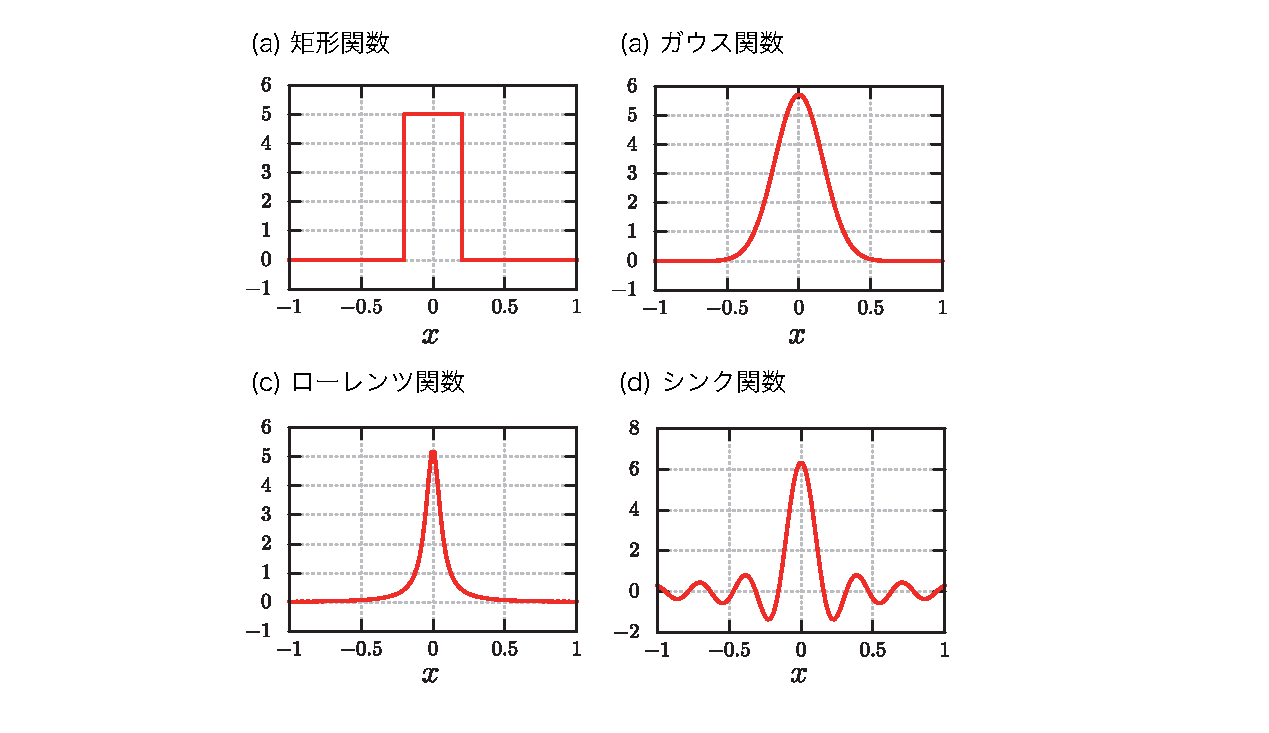
\includegraphics[width=1.0\linewidth]{/Users/kasa/GitHub/lectures/osaka-u/2021/kaenI/chap02_fr/figures/delta-func_explicit.eps} 
\end{figure}
%
\subsection{3次元空間のデルタ関数}
%
3次元空間
${\bf r} = (x,y,z)^{T}$ ($T$は転置を表す)
に対するデルタ関数$\delta\left({\bf r}\right)$は,
\begin{align}
 \delta\left({\bf r}\right) = \delta\left(x\right) \delta\left(y\right) \delta\left(z\right), 
\end{align}
で定義される.
%
%
\section{フーリエ変換}
%
再度,フーリエ積分の式\Eq{fourier_integral}を示しておく(ただし,変数$u$を$k$に変えている).
\begin{align}
 f\left(x\right) = \dfrac{1}{2\pi}\int_{-\infty}^{\infty}dk\,
                    \underline{\left(\int_{-\infty}^{\infty}dx^{\prime}\,f\left(x^{\prime}\right)e^{-ikx^{\prime}}\right)}e^{ikx}. \label{fourier_integral_02}
\end{align}
下線部は,フーリエ級数における展開係数$c_n$に対応するものであり,
これは関数$f(x)$に含まれる成分$k$\footnote{ここでは単に成分$k$と読んでいるが,$k$の呼び方は$x$が持つ次元によって名前が異なる.例えば,$x$が長さの次元を持つ場合,$k$を角波数とよび,$x$が時間の次元を持つときには角周波数(角振動数)と呼ぶ.多くの物理の教科書では,角波数と角周波数を$k$と$\omega$で使い分けている.}の波の量を表している.
そこで,$f(x)$から成分$k$の波の量を抽出する操作$\mathcal{F}[f(x)]$をフーリエ変換と呼び,変換後の関数を$F(k)$と表すことにすると,
\begin{align}
 F\left(k\right) = \mathcal{F}\left[f\left(x\right)\right] = \int_{-\infty}^{\infty}dx\, f\left(x\right)e^{-ikx},
\end{align}
である.また,変換して得られた関数$F\left(k\right)$のこと自体をフーリエ変換と呼ぶことがほとんどなので,混乱しないように.
$F\left(k\right)$から元々の関数$f\left(x\right)$に戻す操作のことをフーリエ逆変換$\mathcal{F}^{-1}\left[F(k)\right]$
と呼び,\Eq{fourier_integral_02}から,
\begin{align}
 f\left(x\right) = \mathcal{F}^{-1}\left[F\left(k\right)\right]
 = \dfrac{1}{2\pi} \int_{-\infty}^{\infty}dk\, F\left(k\right)e^{ikx},
\end{align}
である.

このテキストでの$x$座標のことを実空間,
$k$座標のことをフーリエ空間と呼ぶことがしばしばある.
このテキストでも,その名前をこれから使っていくことにする.
%
\subsection{3次元空間でのフーリエ変換}
%
3次元空間${\bf r}$の関数$f\left({\bf r}\right)$のフーリエ変換$F\left({\bf k}\right)$は次式のように表される.
\begin{align}
 F\left({\bf k}\right) &= \int_{-\infty}^{\infty}dx\int_{-\infty}^{\infty}dy \int_{-\infty}^{\infty}dz
                         e^{-ik_x x}e^{-ik_y y}e^{-ik_z z} f\left({\bf r}\right) \notag \\
                       &= \int d{\bf r}e^{-i{\bf k}\cdot {\bf r}}f\left({\bf r}\right).
\end{align}
%
逆変換は次式である.
\begin{align}
 f({\bf r}) &= \dfrac{1}{\left(2\pi\right)^3} \int_{-\infty}^{\infty}dx\int_{-\infty}^{\infty}dy \int_{-\infty}^{\infty}dz
              e^{ik_x x}e^{ik_y y}e^{ik_z z} F\left({\bf k}\right) \notag \\
            &=  \dfrac{1}{\left(2\pi\right)^3} \int_{-\infty}^{\infty}d{\bf k}\,e^{-i{\bf k}\cdot {\bf r}} F\left({\bf k}\right).
\end{align}
%
\subsection{デルタ関数のフーリエ変換}
%
デルタ関数$\delta(x)$は,次のような性質をもつものであった.
\begin{align}
 \int_{-\infty}^{\infty}dx\,\delta\left(x-a\right)f\left(x\right) = f\left(a\right). 
\end{align}
%
デルタ関数をフーリエ変換すると,
\begin{align}
 \int_{-\infty}^{\infty}dx\,e^{-ikx}\delta\left(x-a\right) = e^{-ika},
\end{align}
となる.
%
$a=0$の場合は,
\begin{align}
 \int_{-\infty}^{\infty}dx\,e^{-ikx}\delta\left(x\right) = 1, 
\end{align}
である\footnote{余談だが,知り合いの先生の御子息(小学生)は,「デルタ関数のフーリエ変換は何だ?言ってみろ」と父親から聞かれて,「イチ!」と答えたらしい.そのお子さんにはいつか「$\delta(x-a)$のフーリエ変換は?」と聞いてみたいところだ.}.
%
なので,1のフーリエ逆変換を考えると,
\begin{align}
 \delta\left(x\right) = \dfrac{1}{2\pi}\int_{-\infty}^{\infty}dk\,e^{ikx}, 
\end{align}
が得られる.
%
\subsection{フーリエ変換が持つ性質}
%
フーリエ変換が持つ重要な性質について,以下でまとめておく.
無条件で成り立つわけではない関係式もあるので,それは導出過程で述べていくことにする
\footnote{ただし,ここでの導出は数学的に粗い部分がある.例えば,途中で現れる式の
フーリエ変換可能性などについての議論はいくつかすっ飛ばしている.気になる人はフーリエ解析や応用数学の教科書を参照すると良い.
大体のものに載っているはずである.}.
以下では,$F\left(k\right) = \mathcal{F}\left[f\left(x\right)\right],~G\left(k\right) = \mathcal{F}\left[g\left(x\right)\right]$,また$a,~b$は定数とする.
\begin{itemize}
  \item 線形性 
	\begin{align}
	  \mathcal{F}\left[af\left(x\right) + bg\left(x\right)\right] = aF\left(k\right) + bG\left(k\right)
	\end{align}

  \item 移動性
	\begin{align}
	  \mathcal{F}\left[e^{iax}f\left(x\right)\right] = F\left(k-a\right) \\
	  \mathcal{F}\left[f\left(x-a\right)\right]      = e^{-iak}F\left(k\right)
	\end{align}
  \item 拡大性
	\begin{align}
	  \mathcal{F}\left[f\left(ax\right)\right] = \dfrac{1}{\left|a\right|}F\left(\dfrac{k}{a}\right). 
	\end{align}
  \item 導関数のフーリエ変換 
	\begin{align}
	  \mathcal{F}\left[\dfrac{d^n}{dx^n}f\left(x\right)\right] = \left(ik\right)^{n} F\left(k\right)
	\end{align}
  \item 積分のフーリエ変換
	\begin{align}
	  \mathcal{F}\left[\int_{-\infty}^{x} dt\, f\left(t\right)\right] = \dfrac{1}{ik}F\left(k\right).
	\end{align}
  \item 畳み込み積分のフーリエ変換
	\begin{align}
	  \mathcal{F}\left[\int_{-\infty}^{\infty}dy\,f\left(y\right)g\left(x-y\right)\right] = F\left(k\right)G\left(k\right),
	\end{align}

\end{itemize}
%
\subsubsection{線形性}
フーリエ変換では次の関係が成り立つ.
\begin{align}
 \mathcal{F}\left[af\left(x\right) + bg\left(x\right)\right] = aF\left(k\right) + bG\left(k\right).
\end{align}
これが成り立つのは,積分に線形性があるからである.つまり,
\begin{align}
 \mathcal{F}\left[af(x) + b g(x)\right] 
   &= \int_{-\infty}^{\infty}dx\,\left(af(x)+bg(x)\right)e^{-ikx} \notag \\
   &= a\int_{-\infty}^{\infty}dx\,f(x)e^{-ikx} + b\int_{-\infty}^{\infty}dx\,g(x)e^{-ikx} \notag \\
   &= aF(k) + bG(k).
\end{align}
%
%
\subsubsection{移動性}
%
$a$を定数として,次式が成り立つ.
%
\begin{align}
 \mathcal{F}\left[e^{iax}f\left(x\right)\right] = F\left(k-a\right), \\
 \mathcal{F}\left[f\left(x-a\right)\right]      = e^{-iak}F\left(k\right). 
\end{align}
%
1つ目は次のようにして示せる.
\begin{align}
 \mathcal{F}\left[e^{iax}f\left(x\right)\right] 
 &=\int_{-\infty}^{\infty}dx\,e^{iax}f\left(x\right)e^{-ikx} \notag \\
 &=\int_{-\infty}^{\infty}dx\,f\left(x\right)e^{-i\left(k-a\right)x} \notag \\
 &=F\left(k-a\right). 
\end{align}
2つ目は$X=x-a$と変数変換することで示せる.
\begin{align}
 \mathcal{F}\left[f\left(x-a\right)\right]      
 &= \int_{-\infty}^{\infty}dx\,f\left(x-a\right)e^{-ikx} \notag \\
 &= \int_{-\infty}^{\infty}dX\,f\left(X\right)e^{-ikx-ika} \notag \\
 &= e^{-ika}F\left(k\right).
\end{align}
%
\subsubsection{拡大性}
%
$a$を定数として,次に示す関係式が成り立つ.
\begin{align}
 \mathcal{F}\left[f\left(ax\right)\right] = \dfrac{1}{\left|a\right|}F\left(\dfrac{k}{a}\right). 
\end{align}
%
$X=ax$と変数変換を行うと,$a>0$のとき,
\begin{align}
 \int_{-\infty}^{\infty}dx\,e^{-ikx}f\left(ax\right) 
 & = \dfrac{1}{a} \int_{-\infty}^{\infty}dx\,f\left(X\right)e^{-i(k/a)X} \notag \\
 & = \dfrac{1}{a}F\left(\dfrac{k}{a}\right),
\end{align}
であり,$a<0$のとき
\begin{align}
 \int_{-\infty}^{\infty}dx\,e^{-ikx}f\left(ax\right) 
 & = \dfrac{1}{a} \int_{\infty}^{-\infty}dx\,f\left(X\right)e^{-i(k/a)X} \notag \\
 & = -\dfrac{1}{a}F\left(\dfrac{k}{a}\right),
\end{align}
従って,両方の場合を考慮すると,目的の式を得る.
%
\subsubsection{導関数のフーリエ変換}
%
$f(x)$の導関数のフーリエ変換は次式のように表すことができる.
\begin{align}
 \mathcal{F}\left[\dfrac{d^n}{dx^n}f\left(x\right)\right] = \left(ik\right)^{n} F\left(k\right). 
\end{align}
無条件で成り立つわけではないが,それは導出の過程で述べることにする.
ここでは,1階の導関数の場合
\begin{align}
 \mathcal{F}\left[\dfrac{d}{dx}f\left(x\right)\right] = ik F\left(k\right),
\end{align}
の関係式を示しておくことにする.積の微分法より,
%
\begin{align}
 \mathcal{F}\left[\dfrac{d}{dx}f\left(x\right)\right] 
 &= \int_{-\infty}^{\infty}dx\,\dfrac{d}{dx}f\left(x\right)e^{-ikx} \notag \\
 &= \biggl[f\left(x\right)e^{-ikx}\biggr]_{-\infty}^{\infty} - \int_{-\infty}^{\infty}dx\,f\left(x\right)\dfrac{d}{dx}e^{-ikx} \notag \\ 
 &= \biggl[f\left(x\right)e^{-ikx}\biggr]_{-\infty}^{\infty} + ik \int_{-\infty}^{\infty}dx\,f\left(x\right)e^{-ikx} \notag \\
 &= \biggl[f\left(x\right)e^{-ikx}\biggr]_{-\infty}^{\infty} + ik F(k), 
\end{align}
となる.ここで,$\displaystyle\lim_{x\to \pm \infty}f\left(x\right)=0$という条件を課して,第1項をゼロにすると,目的の式が得られる.\footnote{正確に言うと,$f^{\prime}(x)$がフーリエ変換可能の場合($f^{\prime}(x)$が区分的になめらかで絶対可積分),$\displaystyle\lim_{x\to \pm}f(x) = 0$が成り立つので,目的の式が得られる.}.
$n$階の導関数の場合も全く同じ手続きで導出できる.

導関数が,フーリエ空間上では$F(k)$に$ik$をかけたものに変わるという性質は,
微分方程式を解く上で極めて有効である.
%
\subsubsection{フーリエ変換の微分}
%

フーリエ変換$F(k)$の微分について,次式が成り立つ.
\begin{align}
 \mathcal{F}\left[\left(-ix\right)^{n}f\left(x\right)\right] = \dfrac{d^n}{dk^n}F\left(k\right). 
\end{align}
%
$n=1$の場合を示しておく.
\begin{align}
  \dfrac{d}{dk}F\left(k\right)
  &= \dfrac{d}{dk}\int_{-\infty}^{\infty}dx\,f\left(x\right)e^{-ikx} \notag \\
  &= \int_{-\infty}^{\infty}dx\, \left(-ix\right)f\left(x\right)e^{-ikx} \notag \\
  &= \mathcal{F}\left[-ixf\left(x\right)\right].
\end{align}
$n=2$以降も同様にして示すことが出来る.
%
\subsubsection{積分のフーリエ変換}
%
$\int_{-\infty}^{\infty}dx\,f\left(x\right) = 0$を満たす関数$f(x)$について,次式が成り立つ.
%
\begin{align}
 \mathcal{F}\left[\int_{-\infty}^{x} dt\, f\left(t\right)\right] = \dfrac{1}{ik}F\left(k\right).
\end{align}
%
先ほどと同様,積の微分法から導くことが出来る.
\begin{align}
 \mathcal{F}\left[\int_{-\infty}^{x}dt\,f\left(t\right)\right] 
& = \int_{-\infty}^{\infty}dx\,\left(\int_{-\infty}^{\infty}dt\,f\left(t\right)\right) e^{-ikx} \notag \\
& = \left[\left(\int_{-\infty}^{x}dt\,f\left(t\right)\right)\dfrac{e^{-ikx}}{-ik}\right]_{-\infty}^{\infty}
    + \dfrac{1}{ik}\int_{-\infty}^{\infty}dx\, f\left(x\right)e^{-ikx} \notag \\
& = \dfrac{1}{ik}F\left(k\right). 
\end{align}
2行目の1項目が消えるのは,$\int_{-\infty}^{\infty}dx\,f\left(x\right) = 0$を仮定しているためである.
%
\subsubsection{畳み込み積分のフーリエ変換}
%
次式のような形で表される積分を畳み込み積分または合成積と呼ぶ.
\begin{align}
 I\left(x\right) = \int_{-\infty}^{\infty}dy\,f\left(y\right)g\left(x-y\right). 
\end{align}
また,上式は
\begin{align}
 I\left(x\right) = \int_{-\infty}^{\infty}dy\,f\left(x-y\right)g\left(y\right),
\end{align}
と等価である(変数変換を試してみればすぐ分かる).
%
理学・工学問わず現れる重要な形の積分である.
\footnote{例えば,私が専門とする液体論では,$h({\bf r}) = c\left({\bf r}\right) + \rho \int d{\bf r}^{\prime}\,c\left({\bf r}^{\prime}\right)h\left({\bf r}-{\bf r}^{\prime}\right)$という形の方程式が,液体の微視的状態を記述する上で重要となる.この式にも畳み込み積分が含まれている.}
%
畳み込み積分をフーリエ変換すると,
%
\begin{align}
 \mathcal{F}\left[\int_{-\infty}^{\infty}dy\,f\left(y\right)g\left(x-y\right)\right] = F\left(k\right)G\left(k\right),
\end{align}
%
のように表される.
この式は,畳み込み積分を計算したかったら,$f(x)$と$g(x)$をそれぞれフーリエ変換して,それらの積をとれば良い,
ということを主張するものであり,理論的な式変形だけでなく数値解析上も極めて有用なものである.
一方で,その導出はシンプルである.まず,
\begin{align}
 e^{-ikx} = e^{-ik\left(x-y\right)}e^{-iky}, 
\end{align}
%
と書き換えることを考える.つまり,
%
\begin{align}
 \mathcal{F}\left[I\left(x\right)\right]
 &= \int_{-\infty}^{\infty}dx\,e^{-ikx}\int_{-\infty}^{\infty}dy\,f\left(y\right)g\left(x-y\right) \notag \\
 &= \int_{-\infty}^{\infty}dy\,\left(f\left(y\right)e^{-iky} \underline{\int_{-\infty}^{\infty}dx\,g\left(x-y\right)e^{-ik\left(x-y\right)}}\right),
\end{align}
%
のようにする.下線部は$G\left(k\right)$なので,
\begin{align}
 \mathcal{F}\left[I\left(x\right)\right] 
 &= \int_{-\infty}^{\infty}dy\,f\left(y\right)e^{-iky}G\left(k\right)\notag \\
 &= F\left(k\right)G\left(k\right),
\end{align}
とできて,目的の式を得る.
%
%
\subsubsection{積のフーリエ変換}
%
今度は積$f(x)g(x)$のフーリエ変換を考えてみよう.実は,実空間での関数の積はフーリエ空間上では
畳み込み積分になる.
%
\begin{align}
 \mathcal{F}\left[f\left(x\right)g\left(x\right)\right] = \dfrac{1}{2\pi}\int_{-\infty}^{\infty}dk\, 
              F\left(k^{\prime}\right) G\left(k-k^{\prime}\right). 
\end{align}
つまり,フーリエ変換することで式変形が厄介になる.

この式を導出するには,まず$f(x)$と$g(x)$のどちらかをフーリエ逆変換の形で表しておく.
\begin{align}
  \mathcal{F}\left[f\left(x\right)g\left(x\right)\right]
  &= \int_{-\infty}^{\infty}dx\,e^{-ikx}\left(\dfrac{1}{2\pi}\int_{-\infty}^{\infty}dk^{\prime}\,e^{ik^{\prime}x}F\left(k\right)\right)g\left(x\right). 
\end{align}
次に,$e^{-ikx}e^{ik^{\prime}x} = e^{-i(k-k^{\prime})x}$のように,ひとまとめにすることで,
\begin{align}
  \mathcal{F}\left[f\left(x\right)g\left(x\right)\right]
  &= \dfrac{1}{2\pi}\int_{-\infty}^{\infty}dk^{\prime}\,\left(F\left(k^{\prime}\right)\int_{-\infty}^{\infty}dx\,e^{-i(k-k^\prime)x}g\left(x\right)\right) \notag \\
  &= \dfrac{1}{2\pi}\int_{-\infty}^{\infty}dk^{\prime}\,F\left(k^{\prime}\right)G\left(k-k^{\prime}\right),
\end{align}
を得る.
%
\newpage
\hrule
\reidai
ガウス関数
\begin{align}
  f\left(x\right) = e^{-ax^2}, \quad (a>0)
\end{align}
のフーリエ変換を求めよ.
\vspace*{.2cm}
\hrule
\vspace*{.2cm}
%
$f(x)$のフーリエ変換を$F(k)$とおくと,
\begin{align}
 F(k) & = \int_{-\infty}^{\infty}dx\, e^{-ikx}e^{-ax^2},
\end{align}
である.まず,指数部分は,
\begin{align}
 -ikx - ax^2 = -a\left(x+\dfrac{ik}{2a}\right)^2 -\dfrac{k^2}{4a}, 
\end{align}
のように平方完成出来るので,
\begin{align}
  F\left(k\right)
  &= \int_{-\infty}^{\infty}dx\,\exp\left[-a\left(x+\dfrac{ik}{2a}\right)^2-\dfrac{k^2}{4a}\right] \notag \\
  &= \exp\left(-\dfrac{k^2}{4a}\right) \int_{-\infty}^{\infty}dx\,\exp\left[-a\left(x+\dfrac{ik}{2a}\right)^2\right], 
\end{align}
となる.ガウス積分\footnote{ガウス積分について未習の場合は,公式として受け入れてほしい.心配しなくても,必ず量子力学の講義で学ぶことになる.}
\begin{align}
 \int_{-\infty}^{\infty}dx\,e^{-ax^2} = \sqrt{\dfrac{\pi}{a}}, 
\end{align}
を用いることで,
\begin{align}
  F\left(k\right) = \sqrt{\dfrac{\pi}{a}}\exp\left(-\dfrac{k^2}{4a}\right), 
\end{align}
を得る\footnote{実はこの解法には少しごまかしが入っているが,その点を理解するためには複素関数論の知識が必要となるので,今回はこれで良しとする.もちろん,結果は正しい.}.
%
\newpage
\hrule
\reidai
次の$f(x)$に関する方程式を解け.
\begin{align}
  \int_{-\infty}^{\infty}dy\,f(y)f(x-y) = \sqrt{\dfrac{a}{\pi}}e^{-ax^2} \quad (a>0) 
\end{align}
\hrule
\vspace*{.2cm}

両辺をフーリエ変換すると,
\begin{align}
  \left(F\left(k\right)\right)^2 = e^{-k^2/4a}.
\end{align}
よって,
\begin{align}
  F\left(k\right) = \pm e^{-k^2/8a},
\end{align}
なので,逆変換すると,
\begin{align}
 f\left(x\right) &= \pm \dfrac{1}{2\pi}\int_{-\infty}^{\infty}dk\,e^{ikx}e^{-k^2/8a} \notag \\
                 &= \sqrt{\dfrac{2a}{\pi}}\exp(-2ax^2). 
\end{align}
\setcounter{chapter}{2}
\chapter{ラプラス解析入門}
%
前章でフーリエ変換を学んだ.簡単に振り返っておくと,
周期関数$f(x)$を三角関数のセットで表現するのがフーリエ級数展開,そして
周期無限大の極限をとったものがフーリエ変換なのだった.
%
フーリエ変換には,実空間($x$)上での畳み込み積分が
フーリエ空間($k$)上では単純な2つの関数の積になるなど,理論展開や数値解析を行う上で有用な
性質を持つ.
一方で,物理や化学で現れる時刻$t$の関数$f(t)$の多くは$t>0$で定義されるものであり,
区間$-\infty \sim \infty$の積分で表されるフーリエ変換ではこれらを扱うのは不便である.
本章で学ぶラプラス(Laplace)変換は,フーリエ変換と似たような性質を持ちつつ
$t=0\sim \infty$の区間で定義された関数を扱うのに長けた応用数学的な手法である.
これを数学的に厳格な立場から学んでいこうとすると,
(化学系としては)いささか高度な数学知識が要求されるが,
化学工学を始めとする様々な工学分野で広く使われるようになった結果,
現在ではラプラス変換の道具としての使い方がかなり整備されている.
理論の詳細にこだわらなければ,様々な微分方程式を初等的な式変形によって解くことができる.
本章では,その道具としてのラプラス変換の使い方に重きをおいて解説していくことにする.
%
\section{ラプラス変換・逆変換}
%
\subsection{ラプラス変換}
%
天下り的ではあるが,まずラプラス変換の定義について述べておく.
$t>0$で区分的に連続な関数$f(t)$と\textbf{複素数}$s$に対し,
\begin{align}
 F(s) = \mathcal{L}\left[f\left(t\right)\right] = \int_{0}^{\infty}dt\,f\left(t\right)e^{-st},
\end{align}
で定義される$f(t)$から$F(s)$への変換$\mathcal{L}$のことをラプラス変換と呼ぶ.
加えて,変換された後の関数$F(s)$のこともラプラス変換と呼ぶのが一般的である.
複素数$s$がとりうる値には制限があるのだが,それは例題を通して言及していくことにする.
%
\newpage
%
\hrule
\reidai
関数
\begin{align}
  f(t) = 1,
\end{align}
のラプラス変換を求めよ.
\vspace*{.2cm}
\hrule
\vspace*{.2cm}

ラプラス変換の定義に則ると,
\begin{align}
 F\left(s\right) = \int_{0}^{\infty}dt\,e^{-st} = \left[-\dfrac{1}{s}e^{-st}\right]_{0}^{\infty} \notag \\
                 = -\dfrac{1}{s}\lim_{t\to \infty}e^{-st} + \dfrac{1}{s}, \label{chap03_reidai01} 
\end{align}
である.$s$は複素数なので実数$\alpha,~\beta$を用いて,
\begin{align}
  s = \alpha + i \beta,  
\end{align}
と表せる.今後しばしば$\mathrm{Re}(s)$, $\mathrm{Im}(s)$なる記号を用いるが,
これらはそれぞれ複素数$s$の実部,虚部を表す.つまり今回の場合では,
\begin{align}
 \mathrm{Re}(s) &= \alpha, \\
 \mathrm{Im}(s) &= \beta, 
\end{align}
である.
\Eq{chap03_reidai01}の第1項は,
\begin{align}
  \dfrac{1}{s}\lim_{t\to \infty}e^{-st} = \dfrac{1}{s}\lim_{t\to \infty}e^{-\alpha t}e^{-i\beta t}, 
\end{align}
と表せるので,極限が特定の値に収束するためには,
\begin{align}
  \mathrm{Re}(s) = \alpha > 0, 
\end{align}
とする必要がある.この条件を満たす場合,極限は0に収束するので,ラプラス変換は
\begin{align}
  F(s) = \dfrac{1}{s}, \quad (\mathrm{Re}(s) > 0) 
\end{align}
である.
%
\newpage
%
この例題で見たように,
任意の$s$について,ラプラス変換が存在するわけではなく,とりうる$s$の範囲は$f(t)$に依存する.

ラプラス変換の存在について議論するために,
まず指数位数(exponential order)なるものを導入する.
$f(t)$が指数$\alpha$位の関数であるとは,定数$M,~\alpha$に対して$f(t)$が
\begin{align}
 \left|f(t)\right| \leq M e^{\alpha t}, \quad (0< t < \infty)
\end{align}
を満たすことをいう.
そして,$f(t)$が区分的に連続で指数$\alpha$位の関数であるならば,
$\mathrm{Re}(s)>\alpha$を満たす任意の$s$に対し,ラプラス変換が存在する.
これは,次の不等式を考えることで示せる.
\begin{align}
  \left|\int_{0}^{\infty}dt,f(t)e^{-st}\right| 
    & \leq \int_{0}^{\infty}dt \, \left|e^{-st}\right| \left|f(t)\right| \notag \\
    & = \int_{0}^{\infty}dt \, e^{-\mathrm{Re}(s)t} \left|f(t)\right| \notag \\
    & \leq \int_{0}^{\infty}dt \, e^{-\mathrm{Re}(s)t} Me^{\alpha t} \notag \\
    & = \left[-\dfrac{M}{\mathrm{Re}(s)-\alpha}e^{-\left(\mathrm{Re}(s)-\alpha\right)t}\right]_{0}^{\infty}. 
\end{align}
$\mathrm{Re}(s) - \alpha > 0$であるから,最後の行は有限の値に収束する.従って,
\begin{align}
  \int_{0}^{\infty}dt\,f(t)e^{-st},
\end{align}
も収束する.つまり,確かにラプラス変換が存在する.

ラプラス変換には,
$\mathrm{Re}(s)>\alpha$ではラプラス変換が存在するが,$\mathrm{Re}(s)<\alpha$では存在しないような定数$\alpha$が存在する.
この$\alpha$のことを収束座標と呼び,
複素平面上の$\mathrm{Re}(s)>\alpha$の領域を収束半平面と呼ぶ.
%
\newpage
%
\hrule
\reidai
次の関数$f(t)$のラプラス変換$F(s)$を求めよ.
\begin{enumerate}[(1)]
  \item $f(t)=a$
  \item $f(t)=t^n$
  \item $f(t)=e^{at}$
  \item $f(t)=\sin(at)$
  \item $f(t)=\cos(at)$ 
\end{enumerate}
\hrule
\begin{enumerate}[(1)]
\item  
\begin{align}
  F(s) & = \int_{0}^{\infty}dt\,ae^{-st} = a\int_{0}^{\infty}dt\,e^{-st}
         = \dfrac{a}{s} 
\end{align}
\item
\begin{align}
  F(s) = \int_{0}^{\infty}dt\,t^n e^{-st} 
\end{align}
上式で$st=u$とおくと,
\begin{align}
  F(s) &= \dfrac{1}{s}\int_{0}^{\infty}du\,\left(\dfrac{u}{s}\right)^{n}e^{-u}
        = \dfrac{1}{s^{n+1}}\int_{0}^{\infty}du\,u^n e^{-u} \notag \\
       &= \dfrac{\Gamma(n+1)}{s^{n+1}} 
\end{align}
ただし,$\Gamma(n)$はガンマ関数と呼ばれ,
\begin{align}
  \Gamma(n) = \int_{0}^{\infty}du\, u^{n-1}e^{-u} 
\end{align}
で定義される.$n$が整数のとき,
\begin{align}
  \Gamma(n) = (n-1)! 
\end{align}
であることから,階乗を一般化したものと言える.
\item
\begin{align}
  F(s) &= \int_{0}^{\infty}dt\,e^{at}e^{-st} = \left[ - \dfrac{e^{-(s-a)t}}{s-a} \right]_{0}^{\infty} \notag \\
       &= \dfrac{1}{s-a}
\end{align}
\item
\begin{align}
  F(s) &= \int_{0}^{\infty}dt\,\sin(at)e^{-st} = \int_{0}^{\infty}dt\,\dfrac{e^{iat}-e^{-iat}}{2i}e^{-st} \notag \\
       &= \dfrac{1}{2i}\int_{0}^{\infty}dt\,\left(e^{-(s-ia)t}-e^{-(s+ia)t}\right) \notag \\
       &= \dfrac{a}{s^{2}+a^{2}}
\end{align}
\item (4)とほとんど同じなので,答えだけ記す.
\begin{align}
  F(s) &= \dfrac{s}{s^{2}+a^{2}} 
\end{align}
\end{enumerate}
\newpage
%
\subsection{ラプラス変換が持つ性質}
%
冒頭で述べたように,ラプラス変換はフーリエ変換とよく似た性質を持つ.
ここではそれを紹介する.ただし,以下では
関数$f(t)$ (指数$\alpha$位, $t<0$でゼロ)のラプラス変換をそれぞれ$F(s)$とする.また,$\mathrm{Re}(s)>\alpha$とする.
%
\begin{itemize}
  \item 線形性
	\begin{align}
	  \mathcal{L}\left[af(t)+bg(t)\right] = aF(s) + bG(s).
	  \label{laplace_linear}
	\end{align}
  \item 移動性
	\begin{align}
          \mathcal{L}\left[f(t-a)\Theta(t-a)\right] = e^{-as}F(s), \label{laplace_shift01}\\
          \mathcal{L}\left[e^{at}f(t)\right]   = F(s-a),           \label{laplace_shift02}
	\end{align}
	ただし,$a>0$である.
	$\Theta(t)$はヘヴィサイドの階段(step)関数と呼ばれるものであり,
	次式で定義される.
	\begin{align}
	  \Theta(t) = 
	  \begin{cases}
	    0 & t < 0 \\
            1 & t > 0 
	  \end{cases}.
	\end{align}
  \item 拡大性
	\begin{align}
	  \mathcal{L}\left[\dfrac{1}{a}f\left(\dfrac{t}{a}\right)\right] = F(as), \quad a > 0. 
	\end{align}
  \item 導関数のラプラス変換
	\begin{align}
	  \mathcal{L}\left[\dfrac{d}{dt}f(t)\right] = sF(s) - f(0). \label{laplace_diff0} 
	\end{align}
	$n$階導関数$f^{(n)}(t)$のラプラス変換は
	\begin{align}
	  \mathcal{L}\left[f^{(n)}(t)\right] 
          &= s^n F(s) - s^{n-1}f(0) - s^{n-2}f^{\prime}(0) -\cdots - s f^{(n-2)}(0) - f^{(n-1)}(0), \label{laplace_diff1}
	\end{align}
	である.ラプラス変換をすることで微分演算子が消えるので,微分方程式を解くのに有効な公式である.
  \item 積分のラプラス変換
	\begin{align}
          \mathcal{L}\left[\int_{0}^{t}d\tau\,f(\tau)\right] = \dfrac{1}{s}F(s). \label{laplace_integrate}
	\end{align}
	ラプラス変換をすることで積分が消えるので,積分方程式(方程式の中に積分が含まれる)を解くのに有効な公式である.
  \item 畳み込み積分のラプラス変換
	\begin{align}
	  \mathcal{L}\left[\int_{0}^{t}d\tau\,f(\tau)g(t-\tau)\right] = F(s)G(s). 
	\end{align}
	積分のラプラス変換と同様,積分方程式を解くのに有効である.
	畳み込み積分の定義がフーリエ変換の場合と少し異なることに注意すること.
\end{itemize}
%
\subsubsection{線形性}
%
ラプラス変換では次の関係性が成り立つ.
\begin{align}
  \mathcal{L}\left[af(t)+bg(t)\right] = aF(s) + bG(s). 
\end{align}
これが成り立つのは積分の線形性があるからである.
フーリエ変換の場合と同じなので,証明は省略する.
%
\subsubsection{移動性}
%
定数$a>0$に対し,次式が成り立つ.
\begin{align}
  \mathcal{L}\left[f(t-a)\Theta(t-a)\right] = e^{-as}F(s), \\
  \mathcal{L}\left[e^{at}f(t)\right]   = F(s-a).
\end{align}
第1式の左辺は,
\begin{align}
 \mathcal{L}\left[f(t-a)\Theta(t-a)\right] &= \int_{a}^{\infty}dt\, f(t-a)e^{-st}, 
\end{align}
であり,$\tau=t-a$と変数変換することで,
\begin{align}
 \mathcal{L}\left[f(t-a)\Theta(t-a)\right] 
  &= \int_{0}^{\infty}d\tau \,f(\tau)e^{-s(\tau + a)} \notag \\
  &= e^{-sa}F(s),
\end{align}
となるので,右辺と一致する.
第2式の左辺は,
\begin{align}
  \mathcal{L}\left[e^{at}f(t)\right] 
  &= \int_{0}^{\infty}dt\,e^{at}f(t)e^{-st} \notag \\
  &= \int_{0}^{\infty}dt\,f(t)e^{-(s-a)t} \notag \\
  &= F(s-a), 
\end{align}
となり,右辺と一致する.
%
\subsubsection{拡大性}
%
定数$a>0$に対し,次の関係性が成り立つ.
\begin{align}
 \mathcal{L}\left[\dfrac{1}{a}f\left(\dfrac{t}{a}\right)\right] = F(as). 
\end{align}
左辺に対し$\tau=t/a$と変数変換することで,
\begin{align}
 \mathcal{L}\left[\dfrac{1}{a}f\left(\dfrac{t}{a}\right)\right]
 &= \dfrac{1}{a}\int_{0}^{\infty}dt\,f\left(\dfrac{t}{a}\right)e^{-st} \notag \\
 &= \int_{0}^{\infty}d\tau \, f(\tau)e^{-sa\tau} \notag \\
 &= F(sa),
\end{align}
を得る.
%
\subsubsection{導関数のラプラス変換}
%
$f(t)$の導関数のラプラス変換は次式のように表される.
\begin{align}
  \mathcal{L}\left[\dfrac{d}{dt}f(t)\right] = sF(s) - f(0). 
\end{align}
%
左辺は部分積分により,
\begin{align}
 \mathcal{L}\left[\dfrac{d}{dt}f(t)\right]
 & = \int_{0}^{\infty}dt\, \left(\dfrac{d}{dt}f(t)\right)e^{-st} \notag \\
 & = \left[f(t)e^{-st}\right]_{0}^{\infty} +s \int_{0}^{\infty}dt\, f(t)e^{-st} \notag \\
 & = \lim_{t\to \infty}f(t)e^{-st} - f(0) + sF(s), 
\end{align}
となる.$f(t)$の指数位数$\alpha$は,
\begin{align}
  \mathrm{Re}(s) > \alpha, 
\end{align}
とすると
\begin{align}
  \left|f(t)e^{-st}\right| 
  &\leq e^{-\mathrm{Re}(s)t}Me^{\alpha t} \notag \\
  & = M e^{-(\mathrm{Re}(s)-\alpha)t} \notag \\
  & \xrightarrow{t\to \infty} 0, 
\end{align}
なので,第1項はゼロとなり,目的の式を得る.
%

この証明は$n$階微分$f^{(n)}(t)$のラプラス変換の場合に容易に拡張することが出来る.
ここではその結果のみを記すことにする(各自でやってみると良い).
\begin{align}
 \mathcal{L}\left[f^{(n)}(t)\right] = s^n F(s) - s^{n-1}f(0) - s^{n-2}f^{\prime}(0) - \cdots sf^{(n-2)}(0)-f^{(n-1)}(0). 
\end{align}
%
\subsubsection{積分のラプラス変換}
%
積分のラプラス変換は
\begin{align}
  \mathcal{L}\left[\int_{0}^{t}d\tau\,f(\tau)\right] = \dfrac{1}{s}F(s),
\end{align}
のように表すことができる.
左辺を書き直すと,
\begin{align}
 \mathcal{L}\left[\int_{0}^{t}d\tau\, f(\tau)\right]
 &=\int_{0}^{\infty}dt\,\left(\int_{0}^{\infty}d\tau\,f(\tau)\right)e^{-st} \notag \\
 &=\left[-\dfrac{1}{s}e^{-st}\int_{0}^{t}d\tau\,f(\tau)\right]_{0}^{\infty} 
   +\dfrac{1}{s}\int_{0}^{\infty}dt\,f(t)e^{-st} \notag \\
 &=-\dfrac{1}{s}\lim_{t\to\infty}e^{-st}\int_{0}^{t}d\tau\,f(\tau) + \dfrac{1}{s}F(s), 
\end{align}
となる.ここで,$f(t)$の指数位数$\alpha$に対し,$\mathrm{Re}(s) > \alpha$なので,
\begin{align}
 \left|e^{-st}\int_{0}^{t}d\tau\, f(\tau)\right| 
 & \leq e^{-\mathrm{Re}(s)t}\int_{0}^{t}d\tau\, Me^{\alpha t} \notag \\
 & = e^{-\mathrm{Re}(s)t}\dfrac{M}{\alpha}\left(e^{-\alpha t}-1\right) \notag \\
 & = \dfrac{M}{\alpha}\left(e^{-(\mathrm{Re}(s)-\alpha)t}-e^{-\mathrm{Re}(s)t}\right) \notag \\
 & \xrightarrow{t\to \infty} 0,
\end{align}
となる.従って,第1項の極限はゼロとなり,目的の式を得る.
%
\subsubsection{畳み込み積分のラプラス変換}
%
次式で定義される畳み込み積分(フーリエ変換の場合と少し違うので注意)
\begin{align}
 \int_{0}^{t}d\tau\, f(\tau)g(t-\tau), 
\end{align}
のラプラス変換は
\begin{align}
 \mathcal{L}\left[\int_{0}^{t}d\tau\,f(\tau)g(t-\tau)\right] = F(s)G(s), 
\end{align}
のように,$f(s),~g(s)$それぞれのラプラス変換の積で表される.
ただし,$g(t)$は$t<0$でゼロで,$g(t)$のラプラス変換を$G(s)$とする.
右辺は
\begin{align}
 F(s)G(s) 
 &= \int_{0}^{\infty}ds\,e^{-sx}\int_{0}^{\infty}dy\, e^{-sy}f(x)g(y) \notag \\
 &= \int_{0}^{\infty}\int_{0}^{\infty}dxdy\,e^{-s(x+y)}f(x)g(y),
\end{align}
であるが,ここで$t=x+y$, $\tau=x$と変数変換すると$dxdy = dtd\tau$であるから,
\begin{align}
 F(s)G(s) = \int_{0}^{\infty}dt\int_{0}^{\infty}d\tau\,e^{-st}f(\tau)g(t-\tau), 
\end{align}
である.さらに,$g(t)$は$t<0$でゼロだから,
\begin{align}
 F(s)G(s) = \int_{0}^{\infty}dt\int_{0}^{t}d\tau\, e^{-st}f(\tau)g(t-\tau), 
\end{align}
となり,目的の式を得る.
%
\subsection{ラプラス逆変換}
%
フーリエ変換の場合と同様,ラプラス変換にも逆変換が存在する.
ラプラス変換が$f(t)$から$F(s)$への変換であったのに対し,
逆変換は$F(s)$から$f(t)$への変換
\begin{align}
 f(t) = \mathcal{L}^{-1}\left[F(s)\right], 
\end{align}
を指す.
%
例えば,例題1で見たように,
\begin{align}
  f(t) = 1 \ce{<=>[ラプラス変換][ラプラス逆変換]} F(s) = \dfrac{1}{s}, 
\end{align}
である.
なので,関数$f_1(t),~f_2(t),\cdots,~f_N(t)$のラプラス変換$F_1(s),~F_2(s),\cdots,F_N(s)$が
既知であった場合,ラプラス変換
\begin{align}
 F(s) = a_1 F_1(s) + a_2 F_2(s) + \cdots + a_N F_N(s), 
\end{align}
の逆変換$f(t)$は,ラプラス変換の線形性\Eq{laplace_linear}より
\begin{align}
 f(t) = a_1 f_1 (t) + a_2 f_2(t) + \cdots a_N f_N(t), 
\end{align}
のように求めることができる.

ラプラス逆変換が積分表示でどのような形になるかを結果だけ示しておく.
まず,絶対収束座標なるものを新たに導入する.積分
\begin{align}
 \int_{0}^{\infty}dt\,\left|e^{-st}f(t)\right|, 
\end{align}
が,$\mathrm{Re}(s)>\beta$で収束し,$\mathrm{Re}(s)<\beta$で収束しないとする.
このような$\beta$のことを絶対収束座標と呼ぶ.
ラプラス逆変換は任意の$a>\beta$に対して,
\begin{align}
 f(t) = \dfrac{1}{2\pi i}\int_{a-i\infty}^{a+i\infty}ds\, F(s)e^{st}, 
\end{align}
で表される.この積分はブロムウィッチ(Bromwich)積分と呼ばれている.
ブロムウィッチ積分を用いて逆変換を求めるには,複素関数論の知識が要求される.
しかし,代表的な関数のラプラス変換・逆変換はラプラス解析の教科書に
表(ラプラス変換表)としてまとめられているので,
それと紹介した公式を駆使することで,逆変換を計算できることが多い.
\footnote{と言いつつ,私の専門に関わるある理論(Smoluchowski-Collins-Kimball)に登場する関数は,そのラプラス変換がとても複雑な形をしていて,
未だに逆変換を自分の手で導出することをサボっている.もしかしたら,変換表と諸定理を使って導出出来るのかもしれないが,
その気力が起きないくらいにゴチャゴチャしているので,試す気も起きなかった.ちなみに,導出自体はかなり昔に報告されているので,頑張れば出来るはずではある.}.
このテキストでも簡易版ではあるが,変換表を掲載しておく.
\begin{table}[htbp]
\centering
\renewcommand{\arraystretch}{1.2}
\begin{tabular}{c|c}
\hline
\hline 
$f\left(t\right)$ & $F\left(s\right)$\tabularnewline
\hline 
$1$ & $\dfrac{1}{s}$\tabularnewline
$\dfrac{t^{n-1}}{\left(n-1\right)!}$ & $\dfrac{1}{s^{n}}$\tabularnewline
$\cos\text{\ensuremath{\omega}}t$ & $\dfrac{s}{s^{2}+\omega^{2}}$\tabularnewline
$\sin\omega t$ & $\dfrac{\omega}{s^{2}+\omega^{2}}$\tabularnewline
$\cosh\omega t$ & $\dfrac{s}{s^{2}-\omega^{2}}$\tabularnewline
$\sinh\omega t$ & $\dfrac{\omega}{s^{2}-\omega^{2}}$\tabularnewline
$e^{bt}\sin at$ & $\dfrac{a}{\left(s-b\right)^{2}+a^{2}}$\tabularnewline
$e^{bt}\cos at$ & $\dfrac{a}{\left(s-b\right)^{2}+a^{2}}$\tabularnewline
$\dfrac{t^{n-1}}{\left(n-1\right)!}e^{at}$ & $\dfrac{1}{\left(s-a\right)^{n}}$\tabularnewline
$t\cos at$ & $\dfrac{s^{2}-a^{2}}{\left(s^{2}+a^{2}\right)^{2}}$\tabularnewline
$t\sin at$ & $\dfrac{2sa}{\left(s^{2}+a^{2}\right)^{2}}$\tabularnewline
$\delta\left(t\right)$ & 1\tabularnewline
\hline 
\end{tabular} 
\end{table}
%
\clearpage
%
\hrule
\reidai
ラプラス逆変換
\begin{align}
 \mathcal{L}^{-1}\left[\dfrac{1}{s^n}\right] = \dfrac{t^{n-1}}{(n-1)!}, 
\end{align}
を示せ.
\vspace*{.2cm}
\hrule
\vspace*{.2cm}
%
まず,
\begin{align}
 \mathcal{L}^{-1}\left[\dfrac{1}{s^n}\right] = \mathcal{L}^{-1}\left[\dfrac{1}{s}\dfrac{1}{s^{n-1}}\right], 
\end{align}
のように書き直してみる.すると,積分のラプラス変換\Eq{laplace_integrate}が使えることに気づく.
\begin{align}
 \mathcal{L}^{-1}\left[\dfrac{1}{s^{n}}\right] = \int_{0}^{t}d\tau_{n}\,\mathcal{L}^{-1}\left[\dfrac{1}{s^{n-1}}\right]. 
\end{align}
これをもう一度繰り返すと,
\begin{align}
  \mathcal{L}^{-1}\left[\dfrac{1}{s^{n}}\right] 
  &= \int_{0}^{t}d\tau_{n}\,\mathcal{L}^{-1}\left[\dfrac{1}{s}\dfrac{1}{s^{n-2}}\right] \notag \\
  &= \int_{0}^{t}d\tau_{n}\int_{0}^{\tau_{n}}d\tau_{n-1}\,\mathcal{L}^{-1}\left[\dfrac{1}{s^{n-2}}\right],
\end{align}
となる.この操作を何度も繰り返すことで次式を得る.
\begin{align}
  \mathcal{L}^{-1}\left[\dfrac{1}{s^{n}}\right] = \int_{0}^{t}d\tau_{n}\int_{0}^{\tau_{n}}d\tau_{n-1}\cdots 
     \int_{0}^{\tau_{3}}d\tau_{2}\,\mathcal{L}^{-1}\left[\dfrac{1}{s}\right]. 
\end{align}
ここで,例題1や変換表が示すように,
\begin{align}
 \mathcal{L}^{-1}\left[\dfrac{1}{s}\right] = 1, 
\end{align}
なので,結局,
\begin{align}
  \mathcal{L}^{-1}\left[\dfrac{1}{s^{n}}\right] 
     &= \int_{0}^{t}d\tau_{n}\int_{0}^{\tau_{n}}d\tau_{n-1}\cdots 
     \int_{0}^{\tau_{3}}d\tau_{2} \notag \\
     &= \dfrac{t^{n-1}}{(n-1)!},
\end{align}
となる.
%
\newpage
%
\subsection{ラプラス逆変換の性質}
%
\begin{itemize}
  \item 微分のラプラス逆変換\\
%
ラプラス変換の1階微分について次式が成り立つ.
\begin{align}
 \mathcal{L}^{-1}\left[\dfrac{d}{ds}F(s)\right] = -tf(t). \label{invlaplace_diff} 
\end{align}
%
$n$階導関数$F^{(n)}(s)$については,
\begin{align}
 \mathcal{L}^{-1}\left[F^{(n)}(s)\right] = (-t)^n f(t),
\end{align}
が成り立つ.

この公式によると,$F(s)$をラプラス逆変換が既知の関数$F_{0}(s)$ (ラプラス逆変換は$f_0(t)$)を用いて,
\begin{align}
F(s) = \dfrac{d}{ds}F_{0}(s), 
\end{align}
と書き直すことで,逆変換を$f(t)=-tf_0(t)$と求めることが出来る.

もちろん,これらの公式をラプラス変換の形で,
\begin{align}
  \mathcal{L}\left[-tf(t)\right] &= \dfrac{d}{ds}F(s), \\
  \mathcal{L}\left[(-t)^n f(t)\right] &= F^{(n)}(s), 
\end{align}
と書いても良い.
%
\item 積分のラプラス逆変換


積分のラプラス逆変換は,
\begin{align}
  \mathcal{L}^{-1}\left[\int_{s}^{\infty}du\,F(u)\right] = \dfrac{f(t)}{t}, \label{invlaplace_int01}
\end{align}
と表すことが出来る.先ほどと同様,
\begin{align}
  \mathcal{L}\left[\dfrac{f(t)}{t}\right] = \int_{s}^{\infty}du\,F(u),  \label{invlaplace_int02}
\end{align}
と表しても良い.
%
\end{itemize}
%
\subsubsection{微分のラプラス逆変換}
%
ここでは,ラプラス変換
\begin{align}
 \mathcal{L}\left[-tf(t)\right] = \dfrac{d}{ds}F(s),
\end{align}
を示す.
右辺は,
\begin{align}
 \dfrac{d}{ds}F(s) 
  &= \dfrac{d}{ds}\int_{0}^{\infty}dt\,f(t)e^{-st} \notag \\
  &= \int_{0}^{\infty}dt\,\dfrac{d}{ds}\left(f(t)e^{-st}\right) \notag \\
  &= \int_{0}^{\infty}dt\,(-t)f(t)e^{-st}\notag \\
  &= \mathcal{L}\left[(-t)f(t)\right], 
\end{align}
となるので\footnote{ホントは微分と積分の順序を入れ替えれるかどうか示さなければならないのだが,細かいことは気にしないことにする.},1階微分に関するラプラス変換の公式が示せた.$n$階微分についても全く同じ手続きで導出出来る.
%
\subsubsection{積分のラプラス逆変換}
%
ラプラス変換
\begin{align}
 \mathcal{L}\left[\dfrac{f(t)}{t}\right] = \int_{s}^{\infty}du\,F(u), 
\end{align}
を示す.
右辺は,
\begin{align}
 \int_{s}^{\infty}du\, F(u) 
    & = \int_{s}^{\infty}du\,\int_{0}^{\infty}dt\,e^{-ut}f(t) \notag \\
    & = \int_{0}^{\infty}dt\int_{s}^{\infty}du\, e^{-ut}f(t)  \notag \\
    & = \int_{0}^{\infty}dt\,f(t)\left[-\dfrac{e^{-ut}}{t}\right]_{u=s}^{u=\infty}\notag \\
    & = \int_{0}^{\infty}dt\,\dfrac{f(t)}{t}e^{-st} \notag \\
    & = \mathcal{L}\left[\dfrac{f(t)}{t}\right],
\end{align}
と書き直せるので,目的の式が得られた.
%
\newpage
%
\hrule
\reidai

ラプラス逆変換
\begin{align}
  \mathcal{L}^{-1}\left[\dfrac{s}{(s^2+a^2)^2}\right], 
\end{align}
を求めよ.
\vspace*{.2cm}
\hrule
\vspace*{.2cm}

\begin{align}
  \mathcal{L}^{-1}\left[\dfrac{s}{(s^2+a^2)^2}\right]
  &= -\dfrac{1}{2a}\mathcal{L}^{-1}\left[\dfrac{d}{ds}\left(\dfrac{a}{s^2+a^2}\right)\right].
\end{align}
ラプラス変換表を見ると,
\begin{align}
 \mathcal{L}^{-1}\left[\dfrac{a}{s^2+a^2}\right] = \sin(at), 
\end{align}
なので,微分のラプラス変換より,
\begin{align}
  \mathcal{L}^{-1}\left[\dfrac{s}{(s^2+a^2)^2}\right]
  &= -\dfrac{1}{2a}(-t)\sin(at) \notag \\
  &= \dfrac{t}{2a}\sin(at).
\end{align}
%
\newpage
%
\hrule
\reidai
関数
\begin{align}
 f(t) = \dfrac{\sin(at)}{t}, 
\end{align}
のラプラス変換を求めよ.
\vspace*{.2cm}
\hrule
\vspace*{.2cm}

積分のラプラス逆変換\Eq{invlaplace_int02}を用いることで,
\begin{align}
  \mathcal{L}\left[\dfrac{\sin(at)}{t}\right] 
  &= \int_{s}^{\infty}du\, \mathcal{L}\left[\sin(at)\right] \notag \\
  &= \int_{s}^{\infty}du\, \dfrac{a}{u^2 + a^2} \notag \\
  &= \left[\tan^{-1}\dfrac{u}{a}\right]_{s}^{\infty} = \dfrac{\pi}{2} - \tan^{-1}\dfrac{s}{a}. 
\end{align}

\subsection{ラプラス変換を学ぶ動機 : 線形常微分方程式への応用}
%
ここまで,ラプラス変換・逆変換の性質や計算方法について述べてきたが,
肝心の「何に使えるのか?」については,あんまり触れていなかったので,
ここで明らかにしておこう.
このテキストでは,ラプラス変換を微分方程式の解法に応用することを目標にしている.
まだ,技巧的なことについて解説すべきことがあるが,まずは簡単な線形常微分方程式を例に
ラプラス変換の有効性について見ていこう.

次の微分方程式を考えよう.
\begin{align}
 \dfrac{d^2f}{dt^2} + 4f = 0, \quad f(0)=f_0, \quad \dfrac{df}{dt}\biggr|_{t=0} = f^{\prime}_0. 
\end{align}
1章で私たちはこの方程式の解き方を知っていて,実際に解いてみると,
\begin{align}
  f(t) = f_0 \cos(2t) + \dfrac{f_0^{\prime}}{2}\sin(2t), 
\end{align}
となる.これをラプラス変換を用いて解いてみよう.まず,両辺をラプラス変換する.
導関数のラプラス変換\Eq{laplace_diff1}を用いると,
\begin{align}
  &\mathcal{L}\left[\dfrac{d^2 f}{dt^2}\right] + 4 \mathcal{L}\left[f\right] = 0, \notag \\
  &\rightarrow \left(s^2 F(s)-sf_0-f_0^{\prime}\right) + 4F(s) = 0, \notag \\
  &\rightarrow (s^2+4)F(s) = sf_0 + f_0^{\prime}, \notag \\
  &\rightarrow F(s) = f_0 \dfrac{s}{s^2+4} + f_0^{\prime}\dfrac{1}{s^2+4}. 
\end{align}
このように,微分方程式にラプラス変換を施すと,初等的な代数方程式に変化する.
これを解のラプラス変換$F(s)$について解くことは上で見たように簡単で,あとは逆変換するだけである.
\begin{align}
 f(t) = f_0 \mathcal{L}^{-1}\left[\dfrac{s}{s^2+4}\right] + f_0^{\prime}\mathcal{L}^{-1}\left[\dfrac{1}{s^2+4} \right].
\end{align}
微分方程式が簡単な代数方程式になった分,皺寄せが逆変換にきているのだが,
私たちはラプラス変換表を持っている.表を眺めて,式中に現れている逆変換がないか調べてみる,もしくは
式変形によって表に載っている形に直せないかを検討する.
今回は既に表に載っているので当てはめると,
\begin{align}
 f(t) = f_0 \cos(2t) + \dfrac{f_0^\prime}{2}\sin(2t), 
\end{align}
となり,確かに微分方程式の解になっている.

この例を見て分かるように,ラプラス変換を使った解法は最後の逆変換が実行出来るかどうかにかかっている.
次節からは,ラプラス変換を変換表に載っている形に書き直す技巧について解説する.
%
\newpage
%
%
%\subsection{単根} 
%
%\begin{align}
%F\left(s\right) & =\dfrac{B\left(s\right)}{A\left(s\right)}=b_{n}+\sum_{i=1}^{n}\dfrac{c_{i1}}{s+p_{i}}
%\end{align}
%
%\begin{align}
%f\left(t\right) & =b_{n}\delta\left(t\right)+\sum_{i=1}^{n}c_{i1}e^{-p_{i}t}.
%\end{align}
\section{部分分数展開によるラプラス逆変換}
%
\subsection{一般論}
%
前節で,ラプラス変換を学ぶモチベーションを説明するために,
ラプラス変換を用いた微分方程式の解法を紹介した.
微分方程式の解のラプラス変換$F(s)$の多くは,
\begin{align}
 F\left(s\right) & =\dfrac{B\left(s\right)}{A\left(s\right)}=\dfrac{b_{n}s^{n}+b_{n-1}s^{n-1}+\cdots+b_{0}}{s^{n}+a_{n-1}s^{n-1}+a_{n-2}s^{n-2}+\cdots+a_{0}},
\end{align}
の形をとっている.ここで,$A(s),~B(s)$はそれぞれ分母,分子の多項式を表す.
上式のような形で表される関数のことを有理関数と呼ぶ.
ラプラス変換が有理関数の場合には,式変形により$F(s)$をラプラス変換表に載っているシンプルな式の組み合わせで表せる.
そのことを以下で見ていこう.

$A(s)$は$n$次なので$n$個の根を持つ.
値の異なる根を$p_1,~p_2,\cdots,~p_r$,そしてそれらの多重度を$m_1,~m_2,\cdots,~m_r$とすると\footnote{$n$と$r$の関係は$n=\displaystyle\sum_{i=1}^{r}m_{i}$.},
%
\begin{align}
 A\left(s\right) & =\left(s+p_{1}\right)^{m_{1}}\left(s+p_{2}\right)^{m_{2}}\cdots\left(s+p_{r}\right)^{m_{r}}\notag\\
 & =\prod_{i=1}^{r}\left(s+p_{i}\right)^{m_{i}},
\end{align}
と書き表せる.
$A(s)$をこのような形で表しておけば,$F(s)$を部分分数に展開できる.
%
\begin{align}
 F\left(s\right) & =\dfrac{B\left(s\right)}{A\left(s\right)}=b_{n}+\sum_{i=1}^{r}\sum_{k=1}^{m_{i}}\dfrac{c_{ik}}{\left(s+p_{i}\right)^{k}}. \label{partial_fraction_expansion}
\end{align}
%
この形に直すと,何がありがたいかと言うと,ラプラス変換の移動性\Eq{laplace_shift01}と変換表にある
\begin{align}
 &\mathcal{L}\left[\dfrac{t^{n-1}}{(n-1)!}\right] = \dfrac{1} {s^n}, \\
 &\mathcal{L}\left[\delta(t)\right] = 1,
\end{align}
から,ラプラス逆変換が次のように実行できてしまうのである.
%
\begin{align}
f\left(t\right) & =b_{n}\delta\left(t\right)+\sum_{i=1}^{r}\sum_{k=1}^{m_{i}}\dfrac{c_{ik}}{\left(k-1\right)!}t^{k-1}e^{-p_{i}t}\notag\\
 & =b_{n}\delta\left(t\right)+\sum_{i=1}^{r}e^{-p_{i}t}\left(\sum_{k=1}^{m_{i}}\dfrac{c_{ik}}{\left(k-1\right)!}t^{k-1}\right). 
\end{align}
%
従って,$F(s)$が有理関数の場合には,ラプラス逆変換を求める問題は
部分分数展開\Eq{partial_fraction_expansion}における
係数$c_{ik}$を求める問題に帰着する.
部分分数分解は高校数学でも学ぶものではあるが,係数を求める方法をいくつか紹介する.
%
\subsection{未定係数法}
%
次に示すラプラス変換$F(s)$を例に考える.
\begin{align}
 F(s) = \dfrac{4}{(s+1)^2(s+3)}. 
\end{align}
%
次式のように部分分数展開することを考える.
\begin{align}
 F(s) = \dfrac{c_1}{(s+1)^2} + \dfrac{c_2}{s+1} + \dfrac{c_3}{s+3}. 
\end{align}
%
これは
\begin{align}
 F(s) &= \dfrac{c_1(s+3)+c_2(s+1)(s+3) + c_3(s+1)^2}{(s+1)^2(s+3)} \notag \\
      &= \dfrac{(c_2+c_3)s^2+(c_1+4c_2+2c_3)s+(3c_1+3c_2+c_3)}{(s+1)^2(s+3)}, 
\end{align}
と書き直せるので,元々の式と比較することで,次の連立方程式を得る.
\begin{align}
  &c_2  +  c_3 = 0, \\
  &c_1  + 4c_2 + 2 c_3 = 0, \\
  &3c_1 + 3c_2 +   c_3 = 4, 
\end{align}
これを解くことにより,$c_1=2,~c_2=-1,~c_3=1$を得るので,
\begin{align}
 F(s) = \dfrac{2}{(s+1)^2} - \dfrac{1}{s+1} + \dfrac{1}{s+3}, 
\end{align}
である.従って,ラプラス逆変換$f(t)$は
\begin{align}
 f(t) = e^{-t}(2t - 1) + e^{-3t}, 
\end{align}
である.
%
\subsection{ヘヴィサイドの方法}
%
未定係数法と同じ$F(s)$を例に考える.この場合でも,
\begin{align}
 F(s) = \dfrac{c_1}{(s+1)^2} + \dfrac{c_2}{s+1} + \dfrac{c_3}{s+3}, \label{pfe_ex01} 
\end{align}
と展開することを考える.
まず,両辺に$(s+3)$をかけると,
\begin{align}
 &             (s+3)F(s)          = (s+3)\left(\dfrac{c_1}{(s+1)^2}+\dfrac{c_2}{s+1}\right) + c_3, \notag \\
 &\rightarrow  \dfrac{4}{(s+1)^2} = (s+3)\left(\dfrac{c_1}{(s+1)^2}+\dfrac{c_2}{s+1}\right) + c_3,
\end{align}
となる.$s=-3$を代入することで,$c_3=1$を得る.
次に,\Eq{pfe_ex01}の両辺に$(s+1)^2$をかける.
\begin{align}
 \dfrac{4}{s+3} = c_1 + (s+1)c_2 + \dfrac{(s+1)^2}{s+3}. \label{pfe_ex01_heav01} 
\end{align}
$s=-1$を代入することで,$c_1 = 2$を得る.さらに,上式を$s$で微分すると,
\begin{align}
 -\dfrac{4}{(s+3)^2} = c_2 + (s+1)X(s) + (s+1)^2 Y(s), 
\end{align}
の形になる.$(s+1)X(s)$と$(s+1)^2Y(s)$は$(s+1)^2/(s+3)$の微分により生ずる項であるが,具体的に求める必要はない.
上式に$s=-1$を代入することで,$c_2 = -1$を得るので,未定係数法と同じ結果が得られた.
ヘヴィサイドの方法では,係数を求めるのに連立方程式を解くことを必要としない一方で,微分演算が(場合によっては)必要となる.

%
\subsection{混合法}
%
未定係数法とヘヴィサイドの方法を混合した方法を紹介する.
ここでも,未定係数法やヘヴィサイドの方法と同じ$F(s)$を例にし,同様の部分分数分解を行うことを考える.
%
\begin{align}
 \dfrac{4}{(s+1)^2(s+3)} &=  \dfrac{c_1}{(s+1)^2} + \dfrac{c_2}{s+1} + \dfrac{c_3}{s+3} \notag \\
                         &=  \dfrac{c_1(s+3)+c_2(s+1)(s+3)+c_3(s+1)^2(s+3)}{(s+1)^2(s+3)}.
\end{align}
%
両辺の分子を比較することで,
\begin{align}
 4 = c_1(s+3) + c_2(s+1)(s+3) + c_3(s+1)^2. 
\end{align}
$s=-3$を代入することで$c_3 = 1$,そして
$s=-1$を代入することで$c_1 = 2$を得る.
両辺を$s$で微分することで,
\begin{align}
 0 = c_1 + c_2(s+3) + (s+1)X(s).
\end{align}
これに$s=-1$を代入することで$c_2 = -1$を得る.
この方法では,通分する手間さえかければ,単純な微分演算から係数を決定できる\footnote{研究室の学生さんにヒアリングしてみたところ,混合法が一番計算がラクに感じるようだ.}.
%
\newpage
%
\section{線形定数係数常微分方程式}
%
$y(t)$に関する定数係数の常微分方程式
\begin{align}
 \sum_{k=0}^{n}a_i\dfrac{d^{k}}{dt^{k}}y(t) = \sum_{k=0}^{n}b_{k}\dfrac{d^k}{dt^k}u(t),\quad a_n=1, 
\end{align}
を考える.これをラプラス変換を用いて整理してみよう.$y(t)$と$u(t)$のラプラス変換をそれぞれ$Y(s),~U(s)$とする.
両辺をラプラス変換すると,微分のラプラス変換の公式より,
\begin{align}
   &\sum_{k=0}^{n}a_{k}\left(s^{k}Y\left(s\right)-\sum_{l=1}^{k}s^{k-l}y^{\left(l-1\right)}\left(0\right)\right) =\sum_{k=0}^{n}b_{k}\left(s^{k}U\left(s\right)-\sum_{l=1}^{k}s^{k-l}u^{\left(l-1\right)}\left(0\right)\right), \notag \\
   &\rightarrow \underbrace{\left(\sum_{k=0}^{n}a_{k}s^{k}\right)}_{\equiv A(s)} Y (s) 
    - \sum_{k=0}^{n}\sum_{l=1}^{k}a_{k}s^{k-l}y^{(l-1)}(0) 
   = \underbrace{\left(\sum_{k=0}^{n}b_{k}s^{k}\right)}_{\equiv B(s)}U(s) - \sum_{k=0}^{n}\sum_{l=1}^{k}b_{k}s^{k-l}u^{(l-1)}(0), \notag \\
   &\rightarrow A(s)Y(s) = B(s)U(s) + 
   \underbrace{\sum_{k=0}^{n}\sum_{l=1}^{k}a_{k}s^{k-l}y^{(l-1)}(0) - \sum_{k=0}^{n}\sum_{l=1}^{k}b_{k}s^{k-l}b^{(l-1)}(0)}_{\equiv C(s)}, \notag \\
   &\rightarrow Y(s) = \dfrac{B(s)}{A(s)}U(s) + \dfrac{C(s)}{A(s)}.
\end{align}
これをラプラス逆変換することで,解$y(t)$に関する表式を得る.
\begin{align}
 y(t) = \mathcal{L}^{-1}\left[\dfrac{B(s)U(s)+C(s)}{A(s)}\right]. 
\end{align}
$A(s)$, $B(s)$は微分方程式の係数から決まる関数,$C(s)$は係数と初期値から決まる関数である.
従って,$u(t)$のラプラス変換$U(s)$を計算できれば,上式から$y(t)$を求めることが出来る.
この式そのものが微分方程式を解くのに便利に使える,というわけでは必ずしもないが,定数係数の線形常微分方程式
が(逆変換さえ実行できれば)ラプラス変換により解ける,ということを示すものである.
ここで,
\begin{align}
  G(s) = \dfrac{B(s)}{A(s)},\quad g(t) = \mathcal{L}^{-1}\left[G(s)\right],
\end{align}
を定義すると,畳み込み積分のラプラス変換の公式より,
\begin{align}
 y(t) = \int_{0}^{t}d\tau\,g(t-\tau)u(\tau) + \mathcal{L}^{-1}\left[\dfrac{C(s)}{A(s)}\right], 
\end{align}
と表せる.$g(t)$のことを伝達関数と呼ぶ\footnote{正確には,$G(s)$のことを伝達関数と呼ぶ.}.
%
\newpage
%
\hrule
\reidai
次の微分方程式を解け.ただし,$y(0)=1$とする.
\begin{align}
 \dfrac{d}{dt}y(t) + 3y(t) + \int_{0}^{t}d \tau\, e^{-(t-\tau)}y(\tau) = -e^{-t} 
\end{align}
\hrule
\vspace*{.2cm}

まず,両辺をラプラス変換する.その際,
微分のラプラス変換の公式
\begin{align}
  \mathcal{L}\left[\dfrac{d}{dt}f(t)\right] = sF(s) - f(0), 
\end{align}
畳み込み積分のラプラス変換の公式
\begin{align}
  \mathcal{L}\left[\int_{0}^{\infty}d\tau\,f\left(t-\tau\right)g\left(\tau\right)\right] & =F\left(s\right)G\left(s\right),
\end{align}
を用いることで,
\begin{align}
 & \left(sY\left(s\right)-y\left(0\right)\right)+3Y\left(s\right)+\dfrac{1}{s+1}Y\left(s\right)=-\dfrac{1}{s+1},\notag\\
 & \rightarrow\left(s+3+\dfrac{1}{s+1}\right)Y\left(s\right)=\dfrac{s}{s+1},\notag\\
 & \rightarrow Y\left(s\right)=\dfrac{s}{\left(s+2\right)^{2}},
\end{align}
を得る.
さらに,次のように部分分数分解することを考える.
\begin{align}
 Y(s) = \dfrac{a}{(s+2)^2} + \dfrac{b}{s+2}. 
\end{align}
$a,~b$はどんな方法を使って求めても良いが,ここでは(かなりくどいが)ヘヴィサイドの方法を使う.
まず,両辺に$(s+2)^2$をかけて,
\begin{align}
  s = a + b(s+2), 
\end{align}
となるので,$s=-2$を代入して,$a=-2$を得る.次に,上式を$s$で微分して,
\begin{align}
  b = 1, 
\end{align}
を得る.
従って,
\begin{align}
 Y(s) = -\dfrac{2}{(s+2)^2} + \dfrac{1}{s+1}, 
\end{align}
である.これをラプラス逆変換する.第2項のラプラス変換は既に知っているように,
\begin{align}
 \mathcal{L}^{-1}\left[\dfrac{1}{s+2}\right] = e^{-2t}, 
\end{align}
である.第2項のラプラス変換は,
\begin{align}
 \mathcal{L}^{-1}\left[-\dfrac{2}{(s+2)^2}\right] 
 &= 2\mathcal{L}^{-1}\left[\dfrac{d}{ds}\left(\dfrac{1}{s+2}\right)\right],
\end{align}
と書き直せるので,微分のラプラス逆変換の公式
\begin{align}
 \mathcal{L}^{-1}\left[\dfrac{d}{ds}F(s)\right] = -tf(t), 
\end{align}
を用いて,
\begin{align}
 \mathcal{L}^{-1}\left[-\dfrac{2}{(s+2)^2}\right] 
 &= 2(-t)\mathcal{L}^{-1}\left[\dfrac{1}{s+2}\right] \notag \\
 &= -2te^{-2t},
\end{align}
である.以上より,
\begin{align}
  y(t) = (1-2t)e^{-2t},
\end{align}
である.
%
\newpage
%
\hrule
\reidai
次の微分方程式を解け.
\begin{align}
 \dfrac{d}{dt}y(t) + a y (t) = (1+a^2)\sin t, \quad y(0) = 0 
\end{align}
\hrule
\vspace*{.2cm}

両辺をラプラス変換すると,
\begin{align}
& sY(s) - y(0) + a Y(s) = (1+a^2)\dfrac{1}{s^2 + 1}, \notag \\
& \rightarrow Y(s) = (1+a^2)\dfrac{1}{s+a}\dfrac{1}{s^2+1} \notag \\
& \rightarrow Y(s) = \dfrac{1}{s+a} + \dfrac{a}{s^2+1} - \dfrac{s}{s^2+1}, 
\end{align}
となる.従って,ラプラス逆変換することにより,
\begin{align}
 y(t) = e^{-at} + a \sin t - \cos t, 
\end{align}
を得る.
\vspace*{.2cm}

比較のために,第1章で学んだ常微分方程式の解法を使って解いてみよう.
まず,与えられた微分方程式の両辺に$e^{at}$をかけて,
\begin{align}
  \dfrac{d}{dt}\left(e^{at}y(t)\right) = (1+a^2)e^{at}\sin t. 
\end{align}
両辺を$t=0\sim t$で積分して,
\begin{align}
  e^{at}y(t) - y(0) 
  &= (1+a^2)\int_{0}^{t}d\tau\, e^{at}\sin t \notag \\
  &= (1+a^2)\dfrac{e^{at}(a\sin t - \cos t) + 1}{1+a^2} \notag \\
  &= e^{at}(a\sin t - \cos t) + 1.
\end{align}
両辺に$e^{-at}$をかけることで,
\begin{align}
  y(t) = e^{at} + a\sin t -\cos t, 
\end{align}
となり,ラプラス変換を使って求めたものと同じ解を得る.
両解法で異なるのは,解を求める過程で積分を実行する必要があるか否かである.
大体の場合,代数的な計算の方が楽なので,ラプラス逆変換を知っている場合はラプラス変換を用いて解く方が計算が楽になる.
%
\newpage
%
\section{ラプラス逆変換しなくても分かること}
%
これまで,
方程式の解のラプラス変換の表式をまず求め,その後に逆変換を実行することで解を得る,
という手続きをとってきた.
しかし,今求めたいものが解$y(t)$そのものではなく,
例えば初期値$y(0)$や$t\to\infty$での値(最終値, $y(\infty)$)だった場合,
ラプラス逆変換を実行しなくてもこれらの情報を得ることが出来る.
%
\subsection{初期値の定理}
関数$f(t)$のラプラス変換を$F(s)$とすると,初期値$f(0)$とラプラス変換$F(s)$の間には
次の関係式が成り立つ.
\begin{align}
 f(0) = \lim_{s\to \infty}sF(s). 
\end{align}
これを初期値の定理と呼ぶ.

これは微分のラプラス変換の公式より,
\begin{align}
  \lim_{s\to\infty}\left(sF(s)-f(0)\right)
  &=\lim_{s\to\infty}\left(\int_{0}^{\infty}dt\,\left(\dfrac{d}{dt}f(t)\right)e^{-st}\right) \notag \\
  &=\int_{0}^{\infty}dt\,\left(\dfrac{d}{dt}f(t)\right)\left(\lim_{s\to \infty}e^{-st}\right) \notag \\
  &= \int_{0}^{\infty}dt\,\left(\dfrac{d}{dt}f(t)\right)\times 0 \notag \\
  &=0,
\end{align}
と出来ることから導かれる.
%
\subsection{最終値の定理}
%
関数$f(t)$のラプラス変換を$F(s)$とすると,最終値$f(\infty)$とラプラス変換$F(s)$の間には
次の関係式が成り立つ.
\begin{align}
 f(\infty) = \lim_{s\to 0}sF(s). 
\end{align}
これを最終値の定理と呼ぶ.
初期値の定理と同様,微分のラプラス変換の公式から,

\begin{align}
  \lim_{s\to0}\left(sF(s)-f(0)\right)
  &=\lim_{s\to 0}\left(\int_{0}^{\infty}dt\,\left(\dfrac{d}{dt}f(t)\right)e^{-st}\right) \notag \\
  &=\int_{0}^{\infty}dt\,\left(\dfrac{d}{dt}f(t)\right)\left(\lim_{s\to 0}e^{-st}\right) \notag \\
  &= \int_{0}^{\infty}dt\,\left(\dfrac{d}{dt}f(t)\right)\times 1 \notag \\
  &=f(\infty)-f(0),
\end{align}
と出来ることから導かれる.
%
%
例えば,ある関数$\rho(r,t)$の$t$に関するラプラス変換$\hat{\rho}(r,s)$が次式のように与えられていたとする.
\begin{align}
 \hat{\rho}(r,s) = \dfrac{1}{s}\left[1-\dfrac{R}{r}\exp\left\{\left(\dfrac{s}{D}\right)^{1/2}(R-r)\right\}\right]. 
\end{align}
$D,~R$は正の定数である.
具体的には述べないが,この関数は実際にある化学反応モデルに登場するものである.
この関数のラプラス逆変換を実行すれば,$\rho(r,t)$が当然得られるわけだが,応用上最もよく使われるのはこの関数の
$t\to \infty$での振る舞いである.
最終値の定理を用いれば,ラプラス逆変換しなくても,
\begin{align}
 \rho(r,\infty) 
  & = \lim_{s\to 0} s\hat{\rho}(r,s) \notag \\
  & = 1- \dfrac{R}{r}, 
\end{align}
と$\rho(r,\infty)$が簡単に求められる.
\chapter{ラプラス変換}
%
%
\end{document}
